\documentclass[a4paper,11pt]{book}
%\documentclass[a4paper,twoside,11pt,titlepage]{book}
\usepackage{listings}
\usepackage[utf8]{inputenc}
\usepackage[spanish]{babel}

% \usepackage[style=list, number=none]{glossary} %
%\usepackage{titlesec}
%\usepackage{pailatino}

\decimalpoint
\usepackage{dcolumn}
\newcolumntype{.}{D{.}{\esperiod}{-1}}
\makeatletter
\addto\shorthandsspanish{\let\esperiod\es@period@code}
\makeatother


%\usepackage[chapter]{algorithm}
\RequirePackage{verbatim}
%\RequirePackage[Glenn]{fncychap}
\usepackage{fancyhdr}
\usepackage{graphicx}
\usepackage{afterpage}

\usepackage{longtable}

\usepackage[pdfborder={000}]{hyperref} %referencia

% ********************************************************************
% Re-usable information
% ********************************************************************
\newcommand{\myTitle}{DETECCIÓN DE PLAGIO EN R\xspace}
\newcommand{\myDegree}{Grado en Ingeniería Informática\xspace}
\newcommand{\myName}{Antonio Javier Rodríguez Pérez\xspace}
\newcommand{\myProf}{Rocío Celeste Romero Zaliz\xspace}
%\newcommand{\mySupervisor}{Put name here\xspace}
\newcommand{\myFaculty}{Escuela Técnica Superior de Ingenierías Informática y de
Telecomunicación\xspace}
\newcommand{\myFacultyShort}{E.T.S. de Ingenierías Informática y de
Telecomunicación\xspace}
\newcommand{\myDepartment}{Departamento de Ciencias de la Computación e Inteligencia Artificial\xspace}
\newcommand{\myUni}{\protect{Universidad de Granada}\xspace}
\newcommand{\myLocation}{Granada\xspace}
\newcommand{\myTime}{\today\xspace}
\newcommand{\myVersion}{Version 0.1\xspace}


\hypersetup{
pdfauthor = {\myName (email (en) antoniojrp@correo.ugr.es)},
pdftitle = {\myTitle},
pdfsubject = {},
pdfkeywords = {palabra_clave1, palabra_clave2, palabra_clave3, ...},
pdfcreator = {LaTeX },
pdfproducer = {pdflatex}
}

%\hyphenation{}


%\usepackage{doxygen/doxygen}
\usepackage{pdfpages}
\usepackage{url}
\usepackage{colortbl,longtable}
\usepackage[stable]{footmisc}
%\usepackage{index}

%\makeindex
%\usepackage[style=long, cols=2,border=plain,toc=true,number=none]{glossary}
% \makeglossary

% Definición de comandos que me son tiles:
%\renewcommand{\indexname}{Índice alfabético}
%\renewcommand{\glossaryname}{Glosario}

\pagestyle{fancy}
\fancyhf{}
\fancyhead[LO]{\leftmark}
\fancyhead[RE]{\rightmark}
\fancyhead[RO,LE]{\textbf{\thepage}}
\renewcommand{\chaptermark}[1]{\markboth{\textbf{#1}}{}}
\renewcommand{\sectionmark}[1]{\markright{\textbf{\thesection. #1}}}

\setlength{\headheight}{1.5\headheight}

\newcommand{\HRule}{\rule{\linewidth}{0.5mm}}
%Definimos los tipos teorema, ejemplo y definición podremos usar estos tipos
%simplemente poniendo \begin{teorema} \end{teorema} ...
\newtheorem{teorema}{Teorema}[chapter]
\newtheorem{ejemplo}{Ejemplo}[chapter]
\newtheorem{definicion}{Definición}[chapter]

\definecolor{gray97}{gray}{.97}
\definecolor{gray75}{gray}{.75}
\definecolor{gray45}{gray}{.45}
\definecolor{gray30}{gray}{.94}

\lstset{ frame=Ltb,
     framerule=0.5pt,
     aboveskip=0.5cm,
     framextopmargin=3pt,
     framexbottommargin=3pt,
     framexleftmargin=0.1cm,
     framesep=0pt,
     rulesep=.4pt,
     backgroundcolor=\color{gray97},
     rulesepcolor=\color{black},
     %
     stringstyle=\ttfamily,
     showstringspaces = false,
     basicstyle=\scriptsize\ttfamily,
     commentstyle=\color{gray45},
     keywordstyle=\bfseries,
     %
     numbers=left,
     numbersep=6pt,
     numberstyle=\tiny,
     numberfirstline = false,
     breaklines=true,
   }
 
% minimizar fragmentado de listados
\lstnewenvironment{listing}[1][]
   {\lstset{#1}\pagebreak[0]}{\pagebreak[0]}

\lstdefinestyle{CodigoC}
   {
	basicstyle=\scriptsize,
	frame=single,
	language=C,
	numbers=left
   }
\lstdefinestyle{CodigoC++}
   {
	basicstyle=\small,
	frame=single,
	backgroundcolor=\color{gray30},
	language=C++,
	numbers=left
   }

 
\lstdefinestyle{Consola}
   {basicstyle=\scriptsize\bf\ttfamily,
    backgroundcolor=\color{gray30},
    frame=single,
    numbers=none
   }


\newcommand{\bigrule}{\titlerule[0.5mm]}


%Para conseguir que en las páginas en blanco no ponga cabecerass
\makeatletter
\def\clearpage{%
  \ifvmode
    \ifnum \@dbltopnum =\m@ne
      \ifdim \pagetotal <\topskip
        \hbox{}
      \fi
    \fi
  \fi
  \newpage
  \thispagestyle{empty}
  \write\m@ne{}
  \vbox{}
  \penalty -\@Mi
}
\makeatother

\usepackage{eurosym} 
\usepackage[section]{placeins}
%\usepackage{pdfpages}
\usepackage{float}
\begin{document}
\begin{titlepage}
 
 
\newlength{\centeroffset}
\setlength{\centeroffset}{-0.5\oddsidemargin}
\addtolength{\centeroffset}{0.5\evensidemargin}
\thispagestyle{empty}

\noindent\hspace*{\centeroffset}\begin{minipage}{\textwidth}

\centering

\includegraphics[width=0.9\textwidth]{imagenes/logo_ugr.jpg}\\[1.4cm]

\textsc{ \Large TRABAJO FIN DE GRADO\\[0.2cm]}
\textsc{ INGENIERÍA EN INFORMÁTICA}\\[1cm]
% Upper part of the page
% 
% Title
{\Huge\bfseries DETECCIÓN DE PLAGIO EN R\\
}
\noindent\rule[-1ex]{\textwidth}{3pt}\\[3.5ex]
%{\large\bfseries Subtitulo del Proyecto}
\end{minipage}

\vspace{2.5cm}
\noindent\hspace*{\centeroffset}\begin{minipage}{\textwidth}
\centering

\textbf{Autor}\\ {Antonio Javier Rodríguez Pérez }\\[2.5ex]
\textbf{Directora}\\
{Rocío Celeste Romero Zaliz}\\[2cm]

\includegraphics[width=0.3\textwidth]{imagenes/etsiit_logo.png}\\[0.1cm]
\textsc{Escuela Técnica Superior de Ingenierías Informática y de Telecomunicación}\\
\textsc{---}\\
Granada,Septiembre de 2018
\end{minipage}
%\addtolength{\textwidth}{\centeroffset}
%\vspace{\stretch{2}}
\end{titlepage}



\chapter*{}
%\thispagestyle{empty}
%\cleardoublepage

\thispagestyle{empty}

\begin{titlepage}
 
 
\setlength{\centeroffset}{-0.5\oddsidemargin}
\addtolength{\centeroffset}{0.5\evensidemargin}
\thispagestyle{empty}

\noindent\hspace*{\centeroffset}\begin{minipage}{\textwidth}

\centering
%
\includegraphics[width=0.9\textwidth]{imagenes/logo_ugr.jpg}\\[1.4cm]

%\textsc{ \Large PROYECTO FIN DE CARRERA\\[0.2cm]}
%\textsc{ INGENIERÍA EN INFORMÁTICA}\\[1cm]
% Upper part of the page
% 

 \vspace{3.3cm}

%si el proyecto tiene logo poner aquí
%
\includegraphics{imagenes/logo.png} 
% \vspace{0.5cm}

% Title

{\Huge\bfseries Detección de Plagio en R\\
}
\noindent\rule[-1ex]{\textwidth}{3pt}\\[3.5ex]
\end{minipage}

\vspace{2.5cm}
\noindent\hspace*{\centeroffset}\begin{minipage}{\textwidth}
\centering

\textbf{Autor}\\ {Antonio Javier Rodríguez Pérez}\\[2.5ex]
\textbf{Directora}\\
{Rocío Celeste Romero Zaliz}\\[2cm]
%
\includegraphics[width=0.15\textwidth]{imagenes/tstc.png}\\[0.1cm]
%\textsc{Departamento de Teoría de la Señal, Telemática y Comunicaciones}\\
%\textsc{---}\\
%Granada, mes de 201
\end{minipage}
%\addtolength{\textwidth}{\centeroffset}
\vspace{\stretch{2}}

 
\end{titlepage}






\cleardoublepage
\thispagestyle{empty}

\begin{center}
{\large\bfseries Detección de Plagio en R}\\
\end{center}
\begin{center}
Antonio Javier Rodríguez Pérez\\
\end{center}

%\vspace{0.7cm}
\noindent{\textbf{Palabras clave}: detección de plagio, analizador léxico, analizador sintáctico, n-grama, algoritmo String Tiling}\\

\vspace{0.7cm}
\noindent{\textbf{Resumen}}\\

El plagio en código fuente y su detección es un problema que encontramos con gran frecuencia en la actualidad dado que hay una gran cantidad de software nuevo y programas en general que se crean cada día.
\newline
Este problema es incluso más preponderante en el ámbito educativo, ya que durante los últimos años se ha convertido en una práctica cada vez más habitual entre los estudiantes.
\newline
Es por esto que es importante que tengamos alguna forma de saber si estos programas son genuinos o tan solo una copia o una modificación de algo ya existente.
\newline
Para detectarlo existen diversas herramientas, pero no existe ninguna creada específicamente para el lenguaje R. 

\vspace{0.3cm}

En este trabajo se busca resolver este problema adaptando una de las herramientas disponibles llamada JPLAG para que funcione también con este lenguaje.
\newline
JPLAG permite determinar con mayor exactitud si existe plagio entre un conjunto de archivos de un mismo lenguaje que se le proporcione.
\newline
Modificar JPLAG para que sirva con R permitirá que la detección de plagio entre programas escritos en este lenguaje sea más rápida y eficiente que con cualquier otro método ya existente.

\cleardoublepage


\thispagestyle{empty}


\begin{center}
{\large\bfseries Plagiarism Detection in R}\\
\end{center}
\begin{center}
Antonio Javier Rodríguez Pérez\\
\end{center}

%\vspace{0.7cm}
\noindent{\textbf{Keywords}: Plagiarism Detection, Parser, Lexer, n-gram, String Tiling Algorithm}\\

\vspace{0.7cm}
\noindent{\textbf{Abstract}}\\

Plagiarism in source code and its detection is a problem we frecuently find nowadays due to the immense amount of new software and programs in general that are made everyday.
\newline
This problem is even more prevalent in the edutational field, since in recent years it has become an increasingly common practice among students.
\newline
For those reasons it's important to have a way of knowing whether that software is genuine or its just a copy or modification of something already existing.
\newline
In order to detect that plagiarism there are many tools avaliable, but there is not yet one created specifically for the language R.

\vspace{0.3cm}

In this proyect we try to solve this issue by adapting one of the avaliable tools called JPLAG so that it'll also function with R.
\newline
JPLAG allows us to determine with great precisión whether there is plagiarism among a set of files written in the same language, that you supply JPLAG with.
\newline
If JPLAG is modified so that it also detects R files, we will be able to detect plagiarism among programs in this language in a faster and more efficient way than any other existing method. 

\chapter*{}
\thispagestyle{empty}

\noindent\rule[-1ex]{\textwidth}{2pt}\\[4.5ex]

Yo, \textbf{Antonio Javier Rodríguez Pérez}, alumno de la titulación Grado en Ingeniería Informática de la \textbf{Escuela Técnica Superior
de Ingenierías Informática y de Telecomunicación de la Universidad de Granada}, con DNI 50643240T, autorizo la
ubicación de la siguiente copia de mi Trabajo Fin de Grado en la biblioteca del centro para que pueda ser
consultada por las personas que lo deseen.

\vspace{6cm}

\noindent Fdo: Antonio Javier Rodríguez Pérez

\vspace{2cm}

\begin{flushright}
Granada a 2 de Septiembre de 2018 .
\end{flushright}


\chapter*{}
\thispagestyle{empty}

\noindent\rule[-1ex]{\textwidth}{2pt}\\[4.5ex]

Dª. \textbf{Rocío Celeste Romero Zaliz}, Profesora del Departamento de Ciencias de la Computación e Inteligencia Artificial de la Universidad de Granada.


\vspace{0.5cm}

\textbf{Informa:}

\vspace{0.5cm}

Que el presente trabajo, titulado \textit{\textbf{DETECCIÓN DE PLAGIO EN R}},
ha sido realizado bajo su supervisión por \textbf{Antonio Javier Rodríguez Pérez}, y autorizo la defensa de dicho trabajo ante el tribunal
que corresponda.

\vspace{0.5cm}

Y para que conste, expide y firma el presente informe en Granada a 2 de Septiembre de 2018 .

\vspace{1cm}

\textbf{La directora:}

\vspace{5cm}

\noindent \textbf{Rocío Celeste Romero Zaliz}

\chapter*{Agradecimientos}
\thispagestyle{empty}

       \vspace{1cm}

Gracias a mi madre y a mi padre, Josefa y Antonio, por insistir en mi educación y ayudarme siempre que lo necesitase.

\bigskip

A mi hermana Laura por sus recomendaciones y por estar siempre ahí.

\bigskip

A Rocío, mi tutora, por guiarme y aconsejarme durante la creación de este proyecto.

\bigskip

A mis amigos de la facultad, con los que he pasado cuatro duros años de estudio. De estos amigos debo mencionar a Javi, Sergio y Jesús ya que son con los que más tiempo he pasado y son los que definen en gran parte quien soy.

\bigskip

Y por último, a Alba, con ella he pasado la mayor parte del tiempo durante estos años de carrera y ha conseguido que vea el mundo de forma diferente.



\chapter*{Declaración de autoría y originalidad del TFG}
\thispagestyle{empty}

Yo, Antonio Javier Rodríguez Pérez, con DNI 50643240T, declaro que el presente documento ha sido realizado por mí y se basa en mi propio trabajo, a menos que se indique lo contrario. No se ha utilizado el trabajo de ninguna otra persona sin el debido reconocimiento. Todas las referencias han sido citadas y todas las fuentes de información y conjuntos de datos han sido específicamente reconocidos.

\vspace{6cm}

\noindent Fdo: Antonio Javier Rodríguez Pérez

\vspace{2cm}

\begin{flushright}
Granada a 2 de Septiembre de 2018 .
\end{flushright}
%\begin{titlepage}
 
 
\setlength{\centeroffset}{-0.5\oddsidemargin}
\addtolength{\centeroffset}{0.5\evensidemargin}
\thispagestyle{empty}

\noindent\hspace*{\centeroffset}\begin{minipage}{\textwidth}

\centering
%
\includegraphics[width=0.9\textwidth]{imagenes/logo_ugr.jpg}\\[1.4cm]

%\textsc{ \Large PROYECTO FIN DE CARRERA\\[0.2cm]}
%\textsc{ INGENIERÍA EN INFORMÁTICA}\\[1cm]
% Upper part of the page
% 

 \vspace{3.3cm}

%si el proyecto tiene logo poner aquí
%
\includegraphics{imagenes/logo.png} 
% \vspace{0.5cm}

% Title

{\Huge\bfseries Detección de Plagio en R\\
}
\noindent\rule[-1ex]{\textwidth}{3pt}\\[3.5ex]
\end{minipage}

\vspace{2.5cm}
\noindent\hspace*{\centeroffset}\begin{minipage}{\textwidth}
\centering

\textbf{Autor}\\ {Antonio Javier Rodríguez Pérez}\\[2.5ex]
\textbf{Directora}\\
{Rocío Celeste Romero Zaliz}\\[2cm]
%
\includegraphics[width=0.15\textwidth]{imagenes/tstc.png}\\[0.1cm]
%\textsc{Departamento de Teoría de la Señal, Telemática y Comunicaciones}\\
%\textsc{---}\\
%Granada, mes de 201
\end{minipage}
%\addtolength{\textwidth}{\centeroffset}
\vspace{\stretch{2}}

 
\end{titlepage}



%\frontmatter
\tableofcontents
\thispagestyle{empty}
\listoffigures
\thispagestyle{empty}
%\listoftables
%
\mainmatter
%\setlength{\parskip}{5pt}

\chapter{Introducción}
 


\section{Un poco de historia}

Plagiar consiste en hacer uso del trabajo o las ideas de otra persona como si fuesen propias \cite{plagio_rae}.
\newline
La palabra plagio proviene del latín "plagiarus" que significa secuestrador y "plaga": "trampa, red" \cite{plagio_etim}. 
\newline
Esta infración empezó a cobrar importancia cuando las palabras e ideas empezaron a ser vistas como propiedad a través de publicaciones . Esto ocurrió a comienzos del siglo dieciocho conforme el arte y la literatura empezaron a verse como expresión de individualidad y personalidad de su autor \cite{plagio_paper}.
\newline
Por esta razón en 1709 se creó la primera ley inglesa de copyright (el Estatuto de la Reina Ana) que con el tiempo fueron incorporando más y más paises en su legislación, siendo Estados Unidos en 1891 el último gran país en incorporar una ley para proteger a sus autores \cite{plagio_historia}.
\newline
En el ámbito académico se procede de distintas formas para penalizar el plagio entre los estudiantes dependiendo de la institución.
\newline
En universidades estadounidenses por ejemplo, las penalizaciones pueden variar dependiendo de si la copia ha sido accidental (reducción de la calificación del estudiante) o intencional. En el caso de ser intencional normalmente se procederá suspendiendo la entrega o la asignatura e incluso expulsando al alumno de la universidad. 
\newline

En el caso de la Universidad de Granada según el Artículo 15 ''Originalidad de los trabajos y pruebas.'' de la normativa de evaluación y de calificación de los estudiantes de la Universidad de Granada, en caso de detectarse plagio esto ''conllevará automáticamente la calificación numérica de cero en la asignatura en la que se hubiera detectado, independientemente del resto de las calificaciones que el estudiante hubiera obtenido'' \cite{normativa_plagio}.
\newline
En la actualidad el plagio también es un problema que ocurre en archivos en código fuente, aunque su detección es más complicada ya que, por ejemplo, la copia se puede producir a nivel de estructura del programa. Además de esto, existen una gran cantidad de lenguajes de programación diferentes con sus características propias y con distintos niveles de abstracción, lo que dificulta aún más su detección ya que naturalmente es necesario que se tengan en cuenta las propias características del lenguaje (sus palabras reservadas, su control de flujo, cómo controlan la creación de objetos,...) a la hora de saber si dos programas escritos en el mismo lenguaje son o no similares.
\newline
Para resolver este problema existen diversas herramientas que automatizan la detección de plagio en código fuente basándose en los "tokens" del lenguaje, el número de veces que se llama a una función, la distancia entre dos secuencias de strings, etc.
\newline
Entre estas herramientas cabe destacar MOSS \cite{Moss_web}, JPLAG \cite{web_jplag}, SIM \cite{sim} y Plaggie \cite{plaggie}.

 
\section{Motivación}

R es un lenguaje de programación de alto nivel y un entorno de software interactivo pensado para computación estadística y gráficas\cite{whatisR}. R está basado en S y en Scheme por lo que también es bastante similar a Matlab.
\newline
R es gratis y de código abierto, no tiene restricciones de licencia, es compatible con Linux, Windows y Macintosh y tiene más de 4800 paquetes con funciones fáciles de usar.
\newline
Por estas razones R es un lenguaje que cada vez más gente usa y se enseña en más y más universidades.
\newline
Aunque su uso se esté expandiendo, todavía no existe una forma para detectar plagio en este lenguaje de forma eficaz y eficiente, ya que ninguna de las herramientas para detección de plagio existentes son compatibles con R tal y como podemos apreciar en la tabla comparativa en la Figura \ref{fig:figura1}. 

\bigskip

\begin{figure}[H] %con el [H] le obligamos a situar aquí la figura
\centering
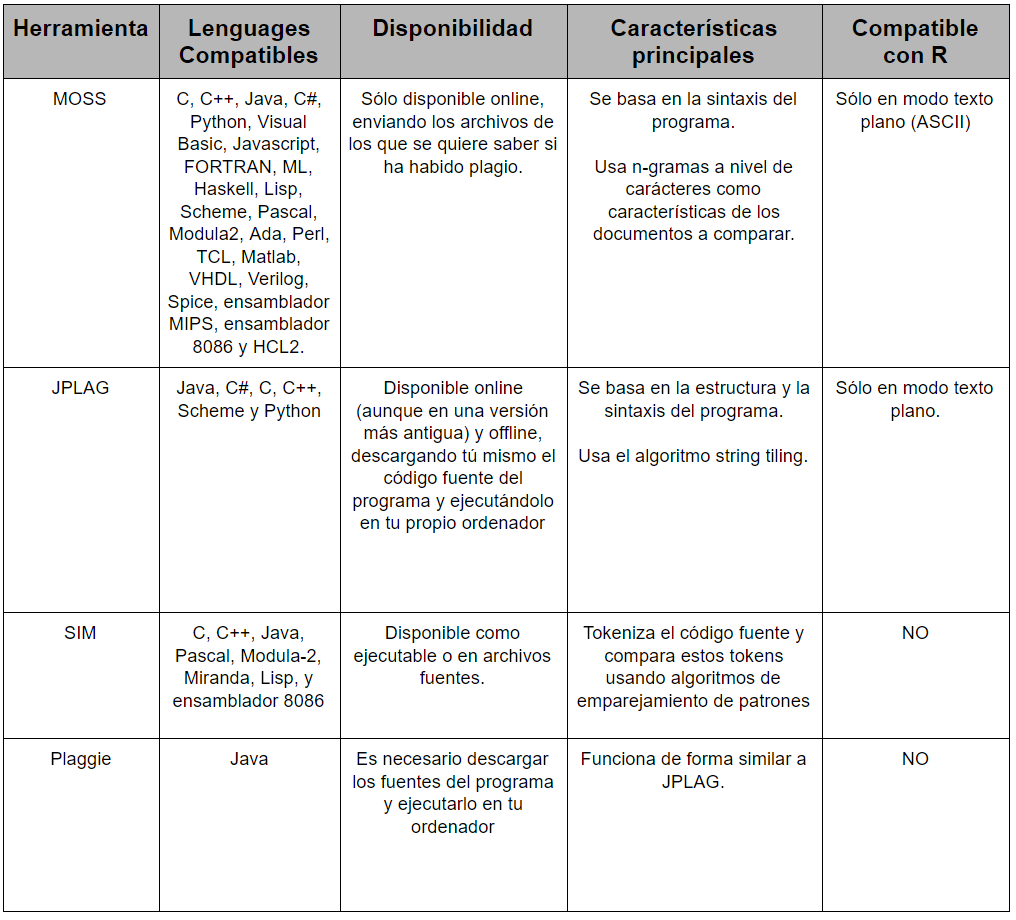
\includegraphics[scale=0.6]{imagenes/tabla_comparativa.png}  %el parámetro scale permite agrandar o achicar la imagen. En el nombre de archivo puede especificar directorios
\caption{Tabla comparativa de las herramientas para detección de plagio en código fuente más prominentes} \label{fig:figura1}
\end{figure}

\bigskip

Dado que, como podemos observar, no existe ninguna herramienta directa para R, hasta el momento lo que se ha hecho es detectarlo de forma manual o usando los detectores de plagio en modo texto plano.
\newline
La detección de forma manual requiere examinar uno a uno los archivos que mandan los alumnos comparándolos entre sí buscando similaridades en el código. Esto es demasiado lento y no efectivo en caso de que haya una gran cantidad de trabajos de alumnos ya que son demasiadas posibles comparaciones como para que el evaluador pueda tener en cuenta lo que han hecho todos los demás.
\newline
Por otra parte usar los detectores de plagio en modo texto plano, aunque sea rápido, pierde en eficacia ya que no tiene en cuenta las características propias del lenguaje y solo detectará plagio en caso de haberse hecho una copia literal.
\newline


\section{Objetivos}

El objetivo por tanto de este trabajo es solucionar este problema adaptando una de las herramientas para detección de plagio disponibles a R.
\newline
Hemos elegido JPLAG como herramienta a adaptar dado que es por norma general la herramienta que da mejores resultados para la detección de plagio en lenguajes en los que sí es compatible y además es la más fácilmente modificable debido a que se estructura en distintos frontends de lenguajes independientes del algoritmo principal de comparación y a que podemos descargar y modificar su código fuente.
\newline
Podemos dividir este objetivo en los siguiente sub-objetivos:
\begin{itemize}
	\item Estudiar y entender el funcionamiento de la estructura de clases de JPLAG
	\item Añadir un frontend para que JPLAG pueda procesar archivos en R.
	\item Modificar dicho frontend para que JPLAG reciba correctamente los "tokens" propios del lenguaje.
	\item Realizar las pruebas necesarias para verificar que se ha adaptado JPLAG correctamente a R y obtiene mejores resultados que en texto plano.
\end{itemize}
	




\section{Estructura del documento}

Este proyecto de fin de grado está estructurado en ocho capítulos que explican todo el trabajo que se ha llevado a cabo para la adaptación de JPLAG a R:
\begin{enumerate}
\item \textbf{Introducción}: en este capítulo se explica el problema en cuestión que queremos resolver.
\item \textbf{Planificación}: organización de mi tiempo y mis recursos para la realización de este trabajo y presupuesto.
\item \textbf{Análisis}: especificación de los requisitos funcionales y no funcionales, y los casos de uso de la tarea en cuestión. 
\item \textbf{Elección de herramientas}: en este capítulo se muestran las herramientas disponibles para la detección de plagio, se explica por qué se han elegido JPLAG y MOSS y se detalla cómo funcionan éstas.
\item \textbf{Implementación}: aquí se explican las partes más importantes del desarrollo, es decir, qué ha sido necesario añadir y modificar para la creación de nuestro frontend y para que éste procese archivos en R.
\item \textbf{Ejecución y Pruebas}: instrucciones sobre cómo ejecutar JPLAG y MOSS, pruebas que se han llevado a cabo con nuestra versión nueva de JPLAG, comparándola con la versión antigua y con MOSS, y análisis de estas pruebas.
\item \textbf{Conclusiones y trabajo futuro}: conclusiones de lo hecho en el trabajo y posibles mejoras que se puedan hacer al frontend.
\item \textbf{Apéndice}: código fuente añadido a JPLAG.
\end{enumerate}

%
\chapter{Planificación}

En este capítulo explico la metodología que se ha seguido para la realización de este trabajo, así como la organización de las tareas hecha siguiendo esta metodología.
\newline
Por último, concluimos este capítulo con el presupuesto del proyecto.


\section{Metodología usada.}

He usado una metodología ágil \cite{metodologia_agil} basándome en SCRUM \cite{scrum}: esta metodología consiste en mantener un contacto frecuente (cada 2 semanas aproximadamente) con nuestro cliente a través de reuniones para revisar el progreso conseguido en la anterior entrega y plantear los objetivos importantes para la próxima. Después de cada reunión se hace un sprint semanal o bisemanal para cumplir los objetivos planteados y se contacta en cualquier momento con el cliente si surge algún problema para replantear el sprint.
\newline
Esta metodología permite que haya un seguimiento del avance mucho más completo, acepta cambios durante cualquier etapa durante el desarrollo y soluciona los errores que surgen de forma más eficaz y con menos presión ya que no hay una entrega general a largo plazo.

En mi caso mi tutora de TFG es mi cliente y las reuniones se han llevado a cabo en su despacho y online (cuando no era posible hablar en persona) cada una o dos semanas dependiendo de la cantidad de trabajo asignada al sprint de la semana actual.


\section{Reparto de objetivos.}

Usando la metodología mencionada en la sección anterior estos han sido las tareas que se han llevado a cabo en cada sprint desde que comencé el trabajo el 4/4/18 hasta el 27/8/18:

\begin{itemize}
	\item \textbf{Primera reunión (4/4/18)}:
	\begin{itemize}
	\item Revisión bibliográfica sobre detección de plagio.
	\item Revisión de software de plagio en código fuente.
	\item Repaso de R.
	\item Búsqueda de software de plagio que funcione con R.
	\end{itemize}
	\item \textbf{Segunda reunión (18/4/18)}:
	\begin{itemize}
	\item Repaso rápido de uso de Latex.
	\item Empezar la redacción del proyecto en Latex.
	\item Ejecución y uso de la versión actual de JPLAG.
	\end{itemize}
	\item \textbf{Tercera reunión (25/4/18)}:
	\begin{itemize}
	\item Especificación de requisitos.
	\item Entender estructura de clases de JPLAG
	\end{itemize}
	\item \textbf{Cuarta reunión (9/5/18)}:
	\begin{itemize}
	\item Adaptar JPLAG para que detecte y use la extensión .r.
	\item Aprender cómo funciona en mayor profundidad Apache Maven para modificar correctamente el archivo pom que usa el proyecto en total.
	\end{itemize}
	\item \textbf{Quinta reunión (16/5/18)}:
	\begin{itemize}
	\item Aprender cómo consigue los tokens de los archivos JPLAG.
	\item Aprender ANTLR4.
	\item Empezar a crear una gramática que define a R para ANTLR4.
	\end{itemize}
	\item \textbf{Sexta reunión (1/6/18)}:
	\begin{itemize}
	\item Estudiar en mayor profundidad la estructura del lenguaje R con sus características específicas para poder crear correctamente su gramática.
	\item Redactar progreso hasta el momento.
	\end{itemize}
	\item \textbf{Séptima reunión (13/6/18)}:
	\begin{itemize}
	\item Crear los archivos .java dentro de nuestro frontend que comunican el parser con JPLAG.
	\item Implementar un parser inicial básico.
	\end{itemize}
	\item \textbf{Octava reunión (20/6/18)}:
	\begin{itemize}
	\item Conectar el parser creado con JPLAG de forma que reciba los tokens de los archivos que analiza.
	\item Elegir los tokens más relevantes del lenguaje (primer intento).
	\end{itemize}
	\item \textbf{Novena reunión (4/7/18)}:
	\begin{itemize}
	\item Realizar prueba inicial con versión actual del frontend.
	\item Redactar en la memoria los avances.
	\end{itemize}
	\item \textbf{Décima reunión (11/7/18)}:
	\begin{itemize}
	\item Modificar la gramática para poder seleccionar tokens más importantes.
	\item Elegir los tokens más relevantes del lenguaje (segundo intento).
	\item Probar de nuevo JPLAG con las modificaciones hechas.
	\end{itemize}
	\item \textbf{Undécima reunión (25/7/18)}:
	\begin{itemize}
	\item Última modificación a la gramática.
	\item Elegir los tokens más relevantes del lenguaje por última vez.
	\item Probar de nuevo JPLAG con las modificaciones hechas con los archivos de alumnos que obtenemos de la tutora.
	\item Anonimizar los archivos de alumnos.
	\end{itemize}
	\item \textbf{Duodécima reunión (6/8/18)}:
	\begin{itemize}
	\item Realizar los benchmarks con todas las entregas de los alumnos con nuestro frontend de R. 
	\item Realizar los benchmarks con todas las entregas de los alumnos con el frontend de texto plano.
	\item Realizar los benchmarks con todas las entregas de los alumnos con MOSS.
	\end{itemize}
	\item \textbf{Trigésima reunión (14/8/18)}:
	\begin{itemize}
	\item Escribir en la memoria la comparación de las pruebas realizadas.
	\item Terminar de redactar la memoria y corregir errores.
	\end{itemize}
	\item \textbf{Cuadragésima reunión (27/8/18)}:
	\begin{itemize}
	\item Últimas mejoras y corrección de errores en la memoria.
	\end{itemize}
\end{itemize}

\section{Presupuesto}

En este apartado planteamos un análisis del valor de los recursos usados para el desarrollo de este proyecto.
\subsection{Recursos materiales}
Aunque las herramientas que hemos estado manipulando para la detección de plagio son gratuitas, hemos hecho uso de una máquina local para realizar todas la pruebas, buscar información y redactar la memoria. Se trata de un ordenador de sobremesa con las siguiente especificaciones:
\begin{itemize}
\item Procesador: Intel i5 4670K (200 \euro)
\item Ram: 8 GB DDR3 (75 \euro)
\item Almacenamiento: HDD 1 TB 7200 rpm (50 \euro)
\item F. alimentación: LC-Power LC600H-12 (44 \euro)
\item Placa base: MSI H81M-P33 (60 \euro)
\item Caja: Aerocool V3XAD (30 \euro) 
\item Sistema Operativo: Windows 10 (proporcionado por la Universidad de Granada)
\end{itemize}
Esto asciende a un total de 459 \euro , aunque a esto hay que añadirle gastos como la electricidad, el material de papelería usado y la conexión a internet. 


\subsection{Recursos humanos}

Teniendo en cuenta que ha sido un trabajo de unos cinco meses de duración con 4 horas de media de trabajo diario 5 días a la semana, tenemos un total de 400 horas de trabajo.
\newline
El salario medio de un ingeniero informático con menos de un año de experiencia es de 17.248\euro  brutos al año.
\newline
400 horas de trabajo equivalen a trabajar durante aproximadamente tres meses por lo que la realización de este trabajo equivale a un total de 4.312\euro.


\subsection{Total}

Juntando los gastos estimados en recursos materiales (600 \euro) y en recursos humanos (4.312 \euro) obtenemos que el coste total aproximado de este proyecto ha sido de 4.912 \euro .




%
%\input{capitulos/03_Planificacion}
%
\chapter{Análisis}

En este capítulo planteo los requisitos funcionales y no funcionales del sistema que he identificado inicialmente y los que han surgido durante su implementación. 
\newline
Así mismo también muestro los actores involucrados en el sistema, un diagrama de los casos de uso y una descripción detallada de cada uno de ellos.



\section{Requisitos Funcionales}
\begin{itemize}
\item \textbf{R.F. 1}. Gestión de Archivos: El sistema debe saber sobre qué archivos debe o no actuar para realizar el análisis del plagio.
	\begin{itemize}
	\item RF 1.1. Se podrán especificar los archivos sobre los que se quiera saber si hay plagio.
	\item RF 1.2. El sistema sabrá reconocer los archivos con extensión .r y .R
	\item RF 1.3. El sistema tiene a R como opción de ejecución para aplicar la detección sobre archivos en este lenguaje. 
	\item RF 1.4. El sistema ignorará los archivos no válidos (que no sean del lenguaje especificado) o con errores.
	\end{itemize}
\item \textbf{R.F. 2}. Gestión de Resultados: El sistema deberá de gestionar los resultados obtenidos de aplicar el algoritmo de JPLAG a los archivos.
	\begin{itemize}
	\item RF 2.1. El sistema guardará los resultados en el directorio que se le especifique.
	\item RF 2.2. El sistema creará los subdirectorios necesarios en caso de no existir la ruta al directorio en el que almacenar los resultados.
	\item RF 2.3. El sistema mostrará los resultados de la ejecución en terminal en todo momento.
	\end{itemize}
\end{itemize}


\section{Requisitos No Funcionales}
\begin{itemize}
\item \textbf{R.N.F. 1}. Eficiencia.
El frontend implantado no deberá demorar en su uso al sistema más que el resto de los frontends para el resto de lenguajes.
\item \textbf{R.N.F. 2}. Eficacia.
El frontend implantado tendrá que obtener resultados iguales o mejores que el resto de frontends con archivos de código en R.
\item \textbf{R.N.F. 3}. Extensivilidad.
El frontend implantado tendrá que ser fácilmente modificable para poder probar con otros tokens del lenguaje.
\end{itemize}

\section{Actores}

\begin{figure}[H] %con el [H] le obligamos a situar aquí la figura
\centering
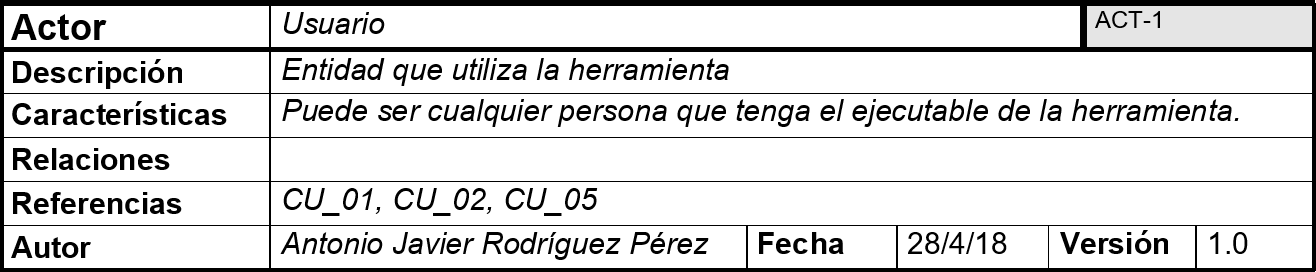
\includegraphics[scale=0.4]{imagenes/ACT_1.png}  %el parámetro scale permite agrandar o achicar la imagen. En el nombre de archivo puede especificar directorios
\caption{Actor 1} \label{fig:figura2}
\end{figure}

\begin{figure}[H] %con el [H] le obligamos a situar aquí la figura
\centering
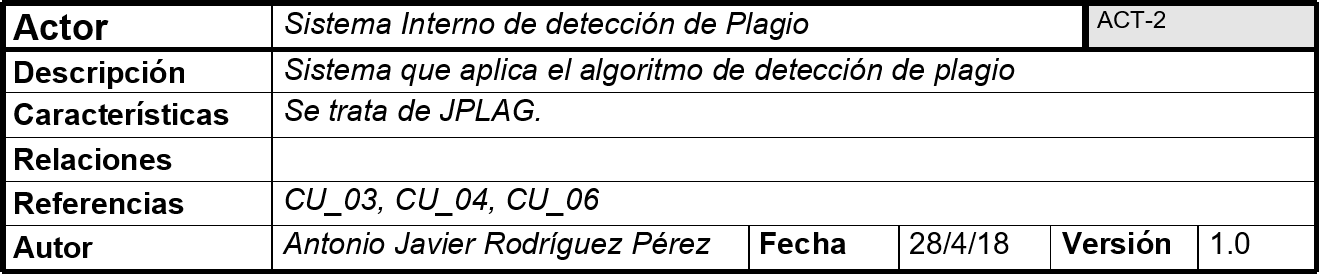
\includegraphics[scale=0.4]{imagenes/ACT_2.png}  %el parámetro scale permite agrandar o achicar la imagen. En el nombre de archivo puede especificar directorios
\caption{Actor 2} \label{fig:figura3}
\end{figure}



\section{Diagrama de Casos de Uso}

\begin{figure}[H] %con el [H] le obligamos a situar aquí la figura
\centering
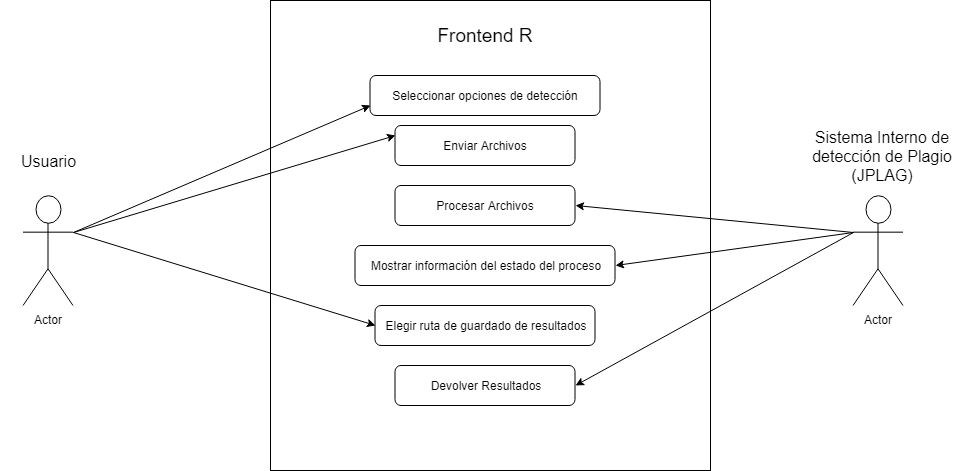
\includegraphics[scale=0.45]{imagenes/Diagrama_CU.png}  %el parámetro scale permite agrandar o achicar la imagen. En el nombre de archivo puede especificar directorios
\caption{Diagrama de casos de uso del usuario del sistema.} \label{fig:figura4}
\end{figure}

\section{Casos de Uso}

\begin{figure}[H] %con el [H] le obligamos a situar aquí la figura
\centering
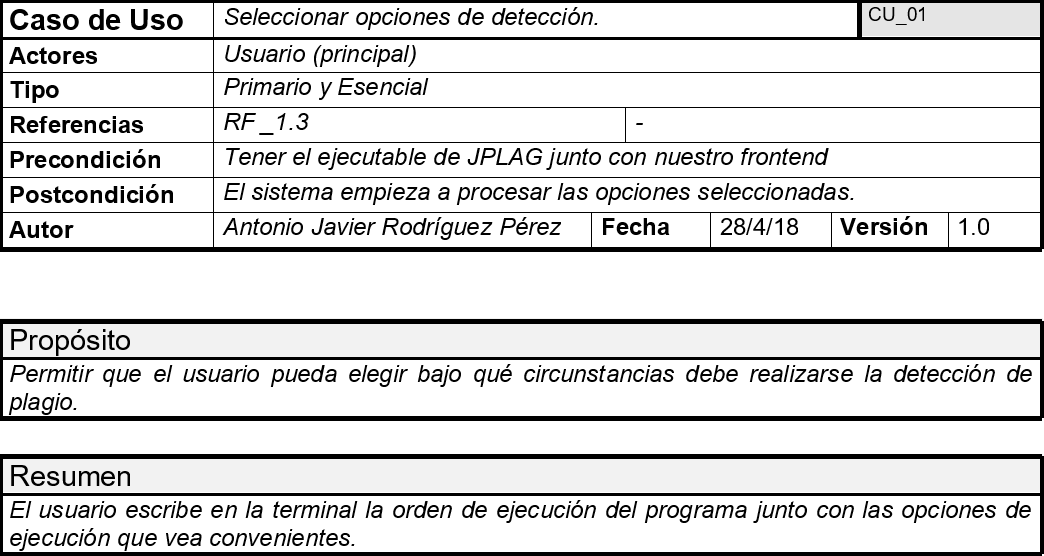
\includegraphics[scale=0.5]{imagenes/CU_01.png}  %el parámetro scale permite agrandar o achicar la imagen. En el nombre de archivo puede especificar directorios
\caption{Caso de uso 1.} \label{fig:CU1}
\end{figure}

\begin{figure}[H] %con el [H] le obligamos a situar aquí la figura
\centering
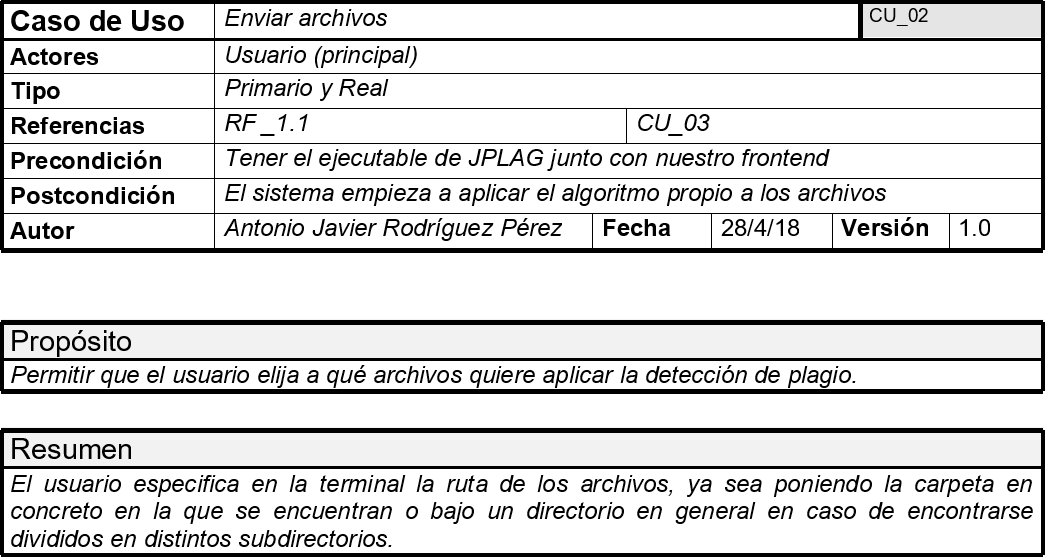
\includegraphics[scale=0.5]{imagenes/CU_02.png}  %el parámetro scale permite agrandar o achicar la imagen. En el nombre de archivo puede especificar directorios
\caption{Caso de uso 2.} \label{fig:CU2}
\end{figure}

\begin{figure}[H] %con el [H] le obligamos a situar aquí la figura
\centering
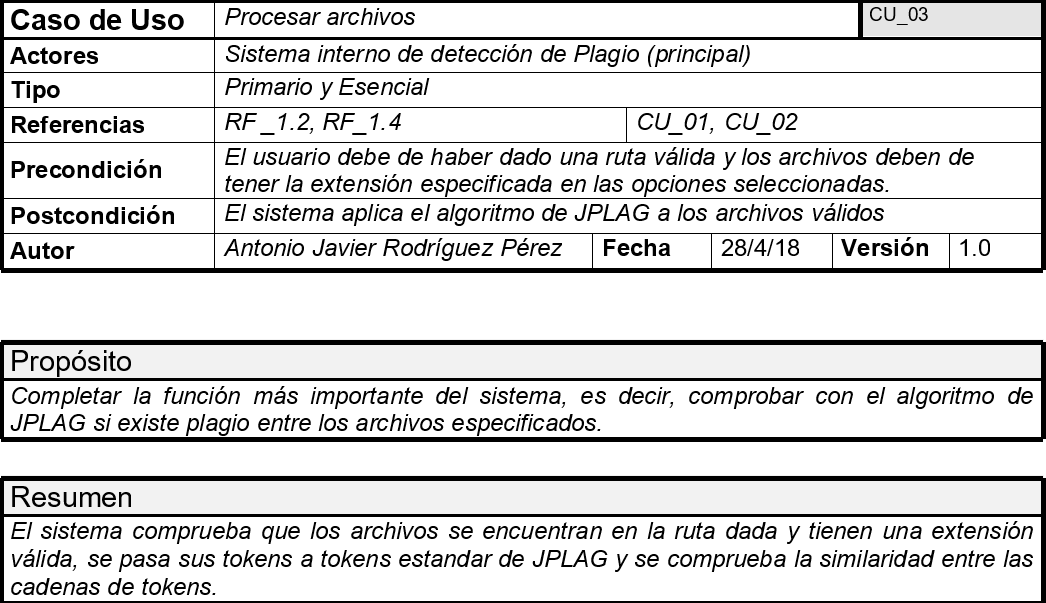
\includegraphics[scale=0.5]{imagenes/CU_03.png}  %el parámetro scale permite agrandar o achicar la imagen. En el nombre de archivo puede especificar directorios
\caption{Caso de uso 3.} \label{fig:CU3}
\end{figure}

\begin{figure}[H] %con el [H] le obligamos a situar aquí la figura
\centering
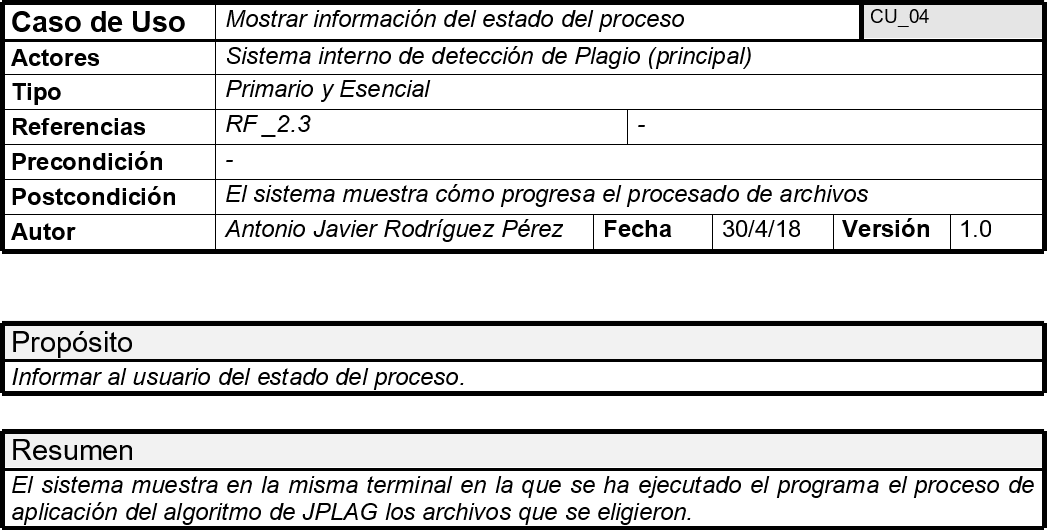
\includegraphics[scale=0.5]{imagenes/CU_04.png}  %el parámetro scale permite agrandar o achicar la imagen. En el nombre de archivo puede especificar directorios
\caption{Caso de uso 4.} \label{fig:CU4}
\end{figure}

\begin{figure}[H] %con el [H] le obligamos a situar aquí la figura
\centering
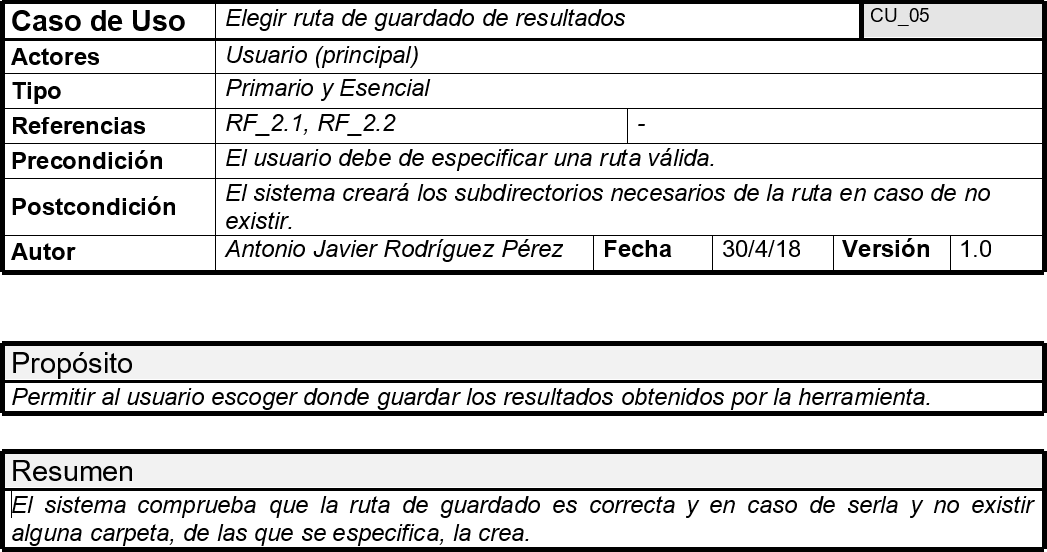
\includegraphics[scale=0.5]{imagenes/CU_05.png}  %el parámetro scale permite agrandar o achicar la imagen. En el nombre de archivo puede especificar directorios
\caption{Caso de uso 5.} \label{fig:CU5}
\end{figure}

\begin{figure}[H] %con el [H] le obligamos a situar aquí la figura
\centering
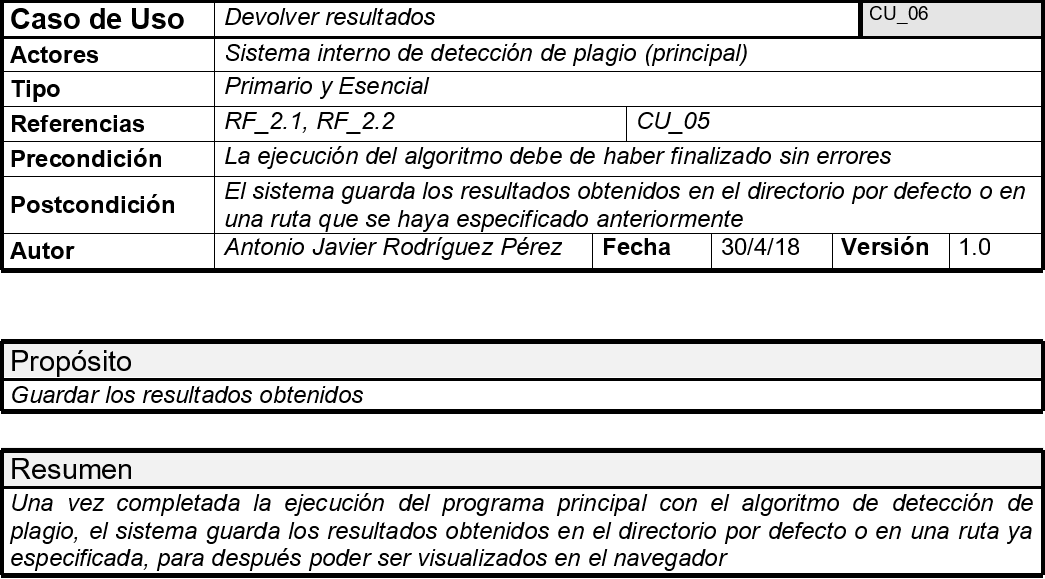
\includegraphics[scale=0.5]{imagenes/CU_06.png}  %el parámetro scale permite agrandar o achicar la imagen. En el nombre de archivo puede especificar directorios
\caption{Caso de uso 6.} \label{fig:CU6}
\end{figure}



\chapter{Elección de herramientas}

\section{Elección de una herramienta base}
En la búsqueda de una herramienta para la detección del plagio encontré diversos servicios como Viper \cite{viper}, Grammarly \cite{grammarly}, Ithenticate \cite{ithenticate}, Plagscan \cite{plagscan} y Turnitin. Entre ellos destaca este último dado que cuenta con una gran base de datos con contenido web, artículos previamente enviados y publicaciones \cite{turnitin}.
\newline
El acceso a estos servicios se hace a través de su interfaz web y está limitado a universidades y otras instituciones o es necesario tener un plan de suscripción de pago.
\newline
Estas herramientas no detectan plagio en sí, sino que devuelven un índice de similaridad entre los archivos enviados y el resto de archivos que tienen en su base de datos.
\newline
Esta similaridad la calculan comparando parámetros como la frecuencia de uso de cada palabra, el parafraseo o la copia literal \cite{plagio_estrategias}.
\newline
Estas herramientas fueron creadas para detectar plagio en trabajos de alumnos escritos en texto plano tales como artículos o memorias de proyectos.
\newline
Es por todo esto que estos servicios no son los más indicados para detectar plagio en archivos de código, a menos que se quiera comprobar si el alumno se ha copiado palabra a palabra de algún archivo de código encontrado online.

\bigskip

Se buscaron por tanto herramientas para la detección de plagio en programas en código fuente.
Existen numerosas herramientas que cumplen ese propósito. En la tabla de la Figura \ref{fig:figura1} muestro las más usadas aunque también debo mencionar: Sherlock \cite{sherlock}, GPlag \cite{gplag}, Marble, Holmes \cite{Moss_Jplag_info} y YAP3 \cite{yap3}. 
\newline
Estos sistemas de detección tienden a adoptar métricas basadas en diferentes aspectos de un archivo de código tales como la complejidad de los flujos de control que se están usando, el número de estructuras de datos que hay de cada tipo, los nombres de las variables y la cantidad de comentarios \cite{plagio_estrategias}.
\newline
Las herramientas que mejores resultados ofrecen y generalmente usan los colegios, universidades, academias y otras instituciones para la detección de plagio entre sus alumnos son MOSS y JPLAG.
\newline
\bigskip
A continuación se explica en qué consiste cada una de estas.


\section{MOSS}

MOSS (Measure Of Software Similarity) es un sistema automático para determinar la similaridad entre programas \cite{Moss_web}, desarrollado en 1994 por Alex Aiken \cite{Moss_uso}, profesor en UC Berlekey en aquel entonces.
\newline
MOSS está disponible como servicio web mediante un servidor que recibe las peticiones que se le envíen a partir de un script en Perl (facilitado por correo automáticamente si lo solicitas). El servidor procesa los archivos enviados con las opciones que se le especifica y devuelve los resultados a través de una interfaz web (devuelve un enlace a los resultados).
\newline
Para proteger la confidencialidad del código de los archivos que se envían al servidor, los resultados generados analizando tal código se borran del servidor 14 días después de su envío.
\newline
Para enviar una petición al servidor tan solo se tendrá que llamar al script usando una opción de comandos similar a la siguiente (partiendo de que el script y los archivos se encuentran en el directorio actual):

\bigskip
\begin{center}
 moss -l matlab *.m
\end{center}
\bigskip

Existen diversas opciones más que podemos usar además de -l. En el primera apartado del capítulo ''Ejecución y Pruebas'' se explican en más detalle.  
\newline
En el siguiente subapartado explicamos en qué consiste su algoritmo de detección.

\subsection{Algoritmo usado}

MOSS se basa en usar n-gramas a nivel de carácter como criterio de comparación entre archivos \cite{Moss_algoritmo}, esta es una ténica comunmente usada en herramientas de detección de plagio. Un n-grama es una subcadena contigua de n elementos, por ejemplo, con n = 5, si tenemos la siguiente cadena en un documento:

\begin{center}
abbcadarrad
\end{center}

Los 5-gramas que se obtienen de esta serán:

\begin{center}
abbca  bbcad  bcada  cadar  adarr  darra  arrad
\end{center}

Una vez obtenidos los n-gramas del documento completo, se le calcula a cada uno un identificador propio (hash) basado en la localización del n-grama en el documento y en los carácteres que lo componen.
\newline
A continuación, se elige un subconjunto de estos hashes para representar al documento (no podemos coger todos los hashes por motivos de eficiencia ya que habrá casi tantos hashes como carácteres en el archivo).
\newline
De esta forma, si la funcion resumen (hash) usada tiene una probabilidad de colisiones pequeña (una colisión consiste en que dos cadenas diferentes tengan la misma función resumen) cuando dos documentos tengan en común algún hash será extremadamente probable que también compartan n-gramas, esto es lo que usa MOSS para calcular similaridad entre programas.
\newline
Para determinar qué funciones resumen escoger normalmente se usa la estrategia de elegir las que sean 0 mod p, para algún p fijo. Esta estrategia es fácil de implementar y nos quedamos únicamente con 1/p de todos los hashes para representar el documento.
\newline
Este método no garantiza que se detecten similaridades entre archivos ya que sólo se detectarán n-gramas iguales cuyo hash sea 0 mod p.
\newline
MOSS soluciona este problema con una técnica llamada windowing (procesar por ventanas).
\newline
En lugar de seleccionar n-gramas aleatorios MOSS selecciona como mínimo una función resumen por cada ventana de un cierto tamaño previamente establecido. Además MOSS usa un valor de n (longitud de n-gramas) grande para evitar ruido en los resultados \cite{Moss_Jplag_info}.

\subsection{Ejemplo de ejecución}
MOSS devuelve los resultados en un enlace que nos lleva a una página con los índices de similaridad entre los archivos enviados tal y como podemos ver en la figura \ref{fig:ej_MOSS1}.
\newline
Si pinchamos en el nombre de algún archivo de los comparados visualizaremos una página en la que se comparan los dos códigos lado a lado como podemos ver en figura \ref{fig:ej_MOSS2}.
En el capítulo de Ejecución y Pruebas se explica con mayor detalle como interpretar estos resultados.

\begin{figure}[H] %con el [H] le obligamos a situar aquí la figura
\centering
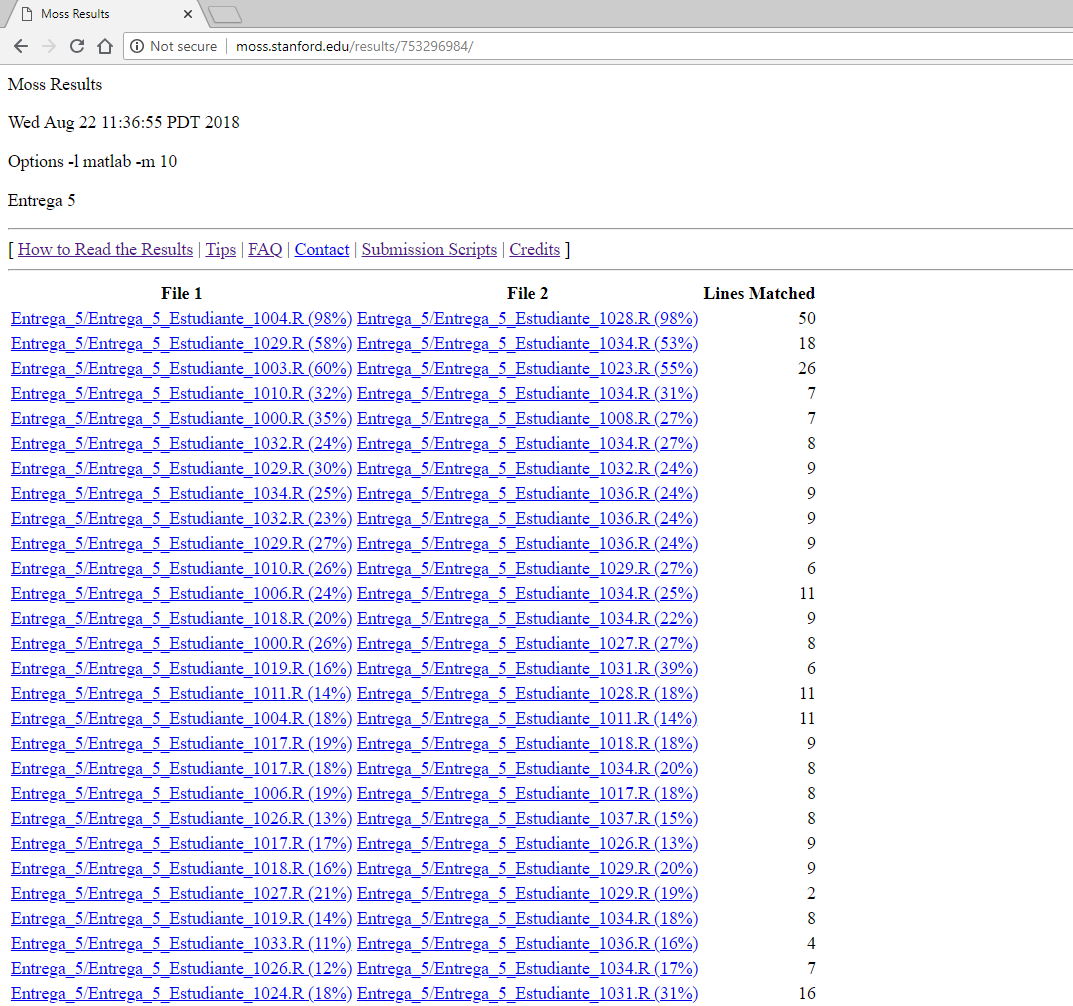
\includegraphics[ width=13cm, height=15cm]{imagenes/MOSS_ejemplo_inicial.png}  %el parámetro scale permite agrandar o achicar la imagen. En el nombre de archivo puede especificar directorios
\caption{Ejemplo de página principal de resultados (MOSS) } \label{fig:ej_MOSS1}
\end{figure}

\begin{figure}[H] %con el [H] le obligamos a situar aquí la figura
\centering
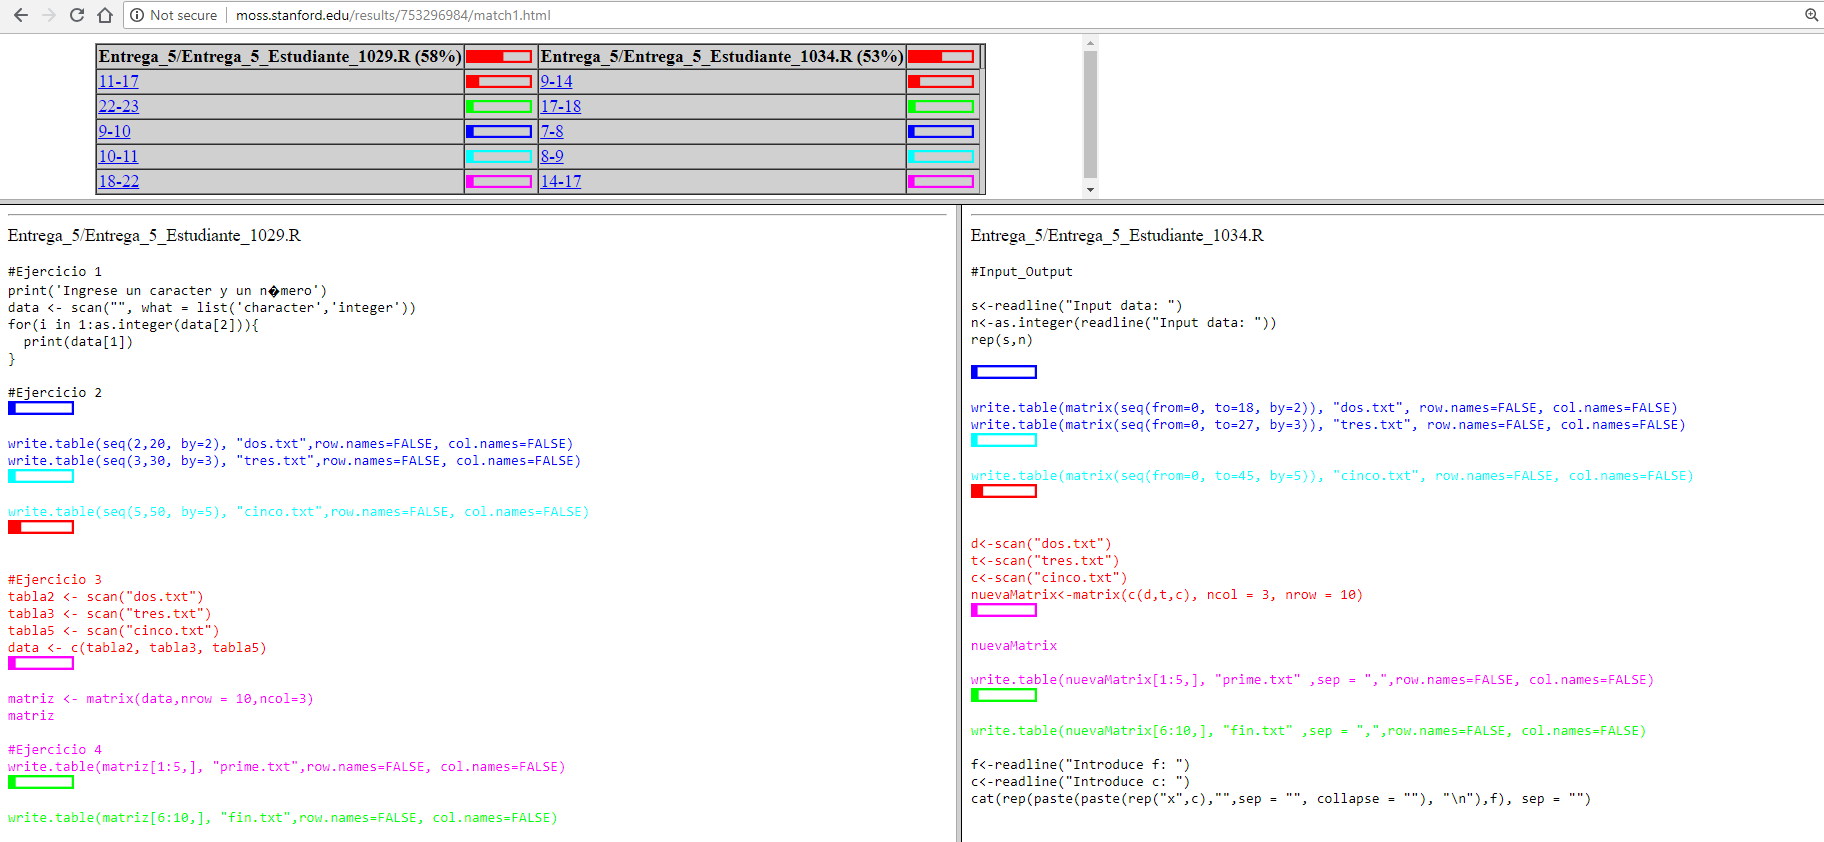
\includegraphics[ height=11cm, width=13cm]{imagenes/MOSS_ejemplo_comparacion.png}  %el parámetro scale permite agrandar o achicar la imagen. En el nombre de archivo puede especificar directorios
\caption{Ejemplo de página de comparación de código de MOSS} \label{fig:ej_MOSS2}
\end{figure}

\section{JPLAG}
JPLAG es un sistema que encuentra similaridades entre conjuntos de archivos en código fuente \cite{web_jplag}. Fue desarrollado por Guido Malpohl en 1996. 
\newline
JPLAG fue creado con la idea de que comparar programas basándose en un vector de características no es suficiente, ya que esto ignora gran parte de la similaridad estructural entre programas \cite{Moss_Jplag_info}. Es por esto que en su lugar intenta emparejar a partir de características estructurales convirtiendo primero el código en una lista de tokens para después aplicar un algoritmo que encuentra emparejamientos entre las listas de tokens obtenidas priorizando emparejamientos lo más largos posible.
\newline
Para usar esta herramienta es necesario descargar su código disponible en Github\cite{jplag_github} y ejecutarlo localmente en nuestro PC. JPLAG genera entonces un conjunto de páginas en HTML con los resultados.
\newline
JPLAG también está disponible como servicio web aunque sus propios desarrolladores no recomiendan su uso ya que usa bibliotecas anticuadas y no está acabado (además de que ya no aceptan nuevos registros).

\subsection{Algoritmo usado}

JPLAG opera en 2 fases \cite{jplag_paper}:
\begin{enumerate}
\item Se analizan sintácticamente o léxicamente(dependiendo del lenguaje) todos los programas enviados, convirtiéndolos en cadenas de tokens.
\item Se comparan las cadenas de tokens por pares.
\end{enumerate}


\subsubsection{1. Análisis Sintáctico}
Esta es la única parte que depende del lenguaje en cuestión en el que están escritos los archivos que se envían a JPLAG. Se trata del frontend de JPLAG.
\newline
El frontend se encarga de realizar un análisis sintáctico o léxico (parser o scanner) de los archivos para reconocer los tokens que los componen como podemos apreciar en la figura \ref{fig:ej_JPLAG1}.

\begin{figure}[H] %con el [H] le obligamos a situar aquí la figura
\centering
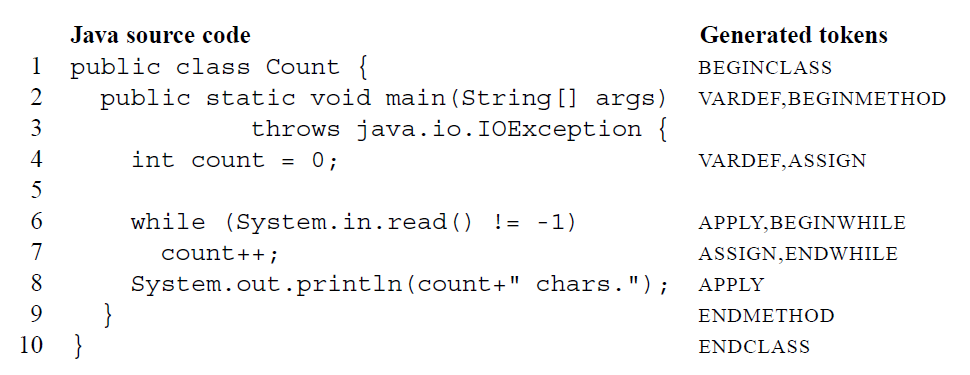
\includegraphics[scale=0.5]{imagenes/JPLAG_ejemplo_tokens.png}  %el parámetro scale permite agrandar o achicar la imagen. En el nombre de archivo puede especificar directorios
\caption{Ejemplo de tokens extraidos de código en java } \label{fig:ej_JPLAG1}
\end{figure}


Los tokens que se escogen deben de ser representativos del lenguaje que estemos tratando para que capturen la esencia del programa (la cual es difícil de cambiar por un plagiador).
\newline
Los espacios en blanco y los comentarios nunca se deben de tener en cuenta como tokens.


\subsubsection{2. Comparación de los tokens}
El algoritmo usado para comparar las cadenas de tokens es básicamente Greedy String Tiling, algoritmo desarrollado por Michael Wise, creador de YAP3, herramienta donde lo aplica \cite{yap3}.
\newline
Cuando se comparan 2 cadenas de tokens deben cumplirse tres reglas:
\begin{enumerate}
\item Un token de una cadena sólo puede ser asociado a un token de la cadena con la que se compara.
\item Las subcadenas de tokens deben de ser independientes de su posición en la cadena principal de tokens. 
\item Tendrán preferencia los emparejamientos largos (de muchos tokens seguidos) sobre los cortos.
\newline
\end{enumerate}

\bigskip
Al aplicar la tercera regla estamos ante un algotimo voraz (greedy) que consiste en tres bucles anidados: el primer bucle itera sobre todos los tokens de la primera cadena (que llamaremos X), el segundo bucle compara el token en el que estamos de X con cada token de la segunda cadena (que llamaremos Y), en caso de ser el mismo token en algún punto del segundo bucle se entra en el tercer bucle, donde se siguen comparando entre X e Y para ver cuántos tokens seguidos son iguales desde ese punto. 
\newline Una vez hecho esto marcamos los emparejamientos de mayor longitud encontrados y repetimos el proceso completo una y otra vez pero sin tener en cuenta en cada vuelta los tokens que ya han sido marcados.
\newline Se repite el proceso hasta que no se encuentre ningún emparejamiento.  

\bigskip
Este es el algoritmo que usa JPLAG con la diferencia de le aplica algunas optimizaciones en tiempo de ejecución. Aunque la complejidad del algoritmo en el peor caso ($\mathcal{O}(n^3)$) no se puede reducir, sí que es posible reducir la complejidad media de los casos prácticos a $\mathcal{O}(n)$.
\newline
Esto es lo que consigue JPLAG adaptando al algoritmo de greedy string tiling la idea del algoritmo de Karp-Rabin \cite{Rabin} en el cual se encuentran ocurrencias de una cadena corta en otra larga usando funciones hash.


\subsection{Ejemplo de ejecución}
JPLAG devuelve los resultados en un conjunto de páginas HTML cuya página principal muestra los mayores índices de similaridad entre los archivos enviados junto con un histograma con todos los índices entre los archivos tal y como podemos ver en la figura \ref{fig:ej_JPLAG2}.
\newline
Si pinchamos en el nombre de algún archivo de los comparados visualizaremos una página en la que se comparan los dos códigos lado a lado como podemos ver en figura \ref{fig:ej_JPLAG3}.
Podemos apreciar que la forma de devolver los resultados de MOSS y JPLAG son muy similares, esto se debe a que la interfaz web de MOSS también la hizo Guido Malpohl(creador de JPLAG) \cite{moss_credits}.

\begin{figure}[H] %con el [H] le obligamos a situar aquí la figura
\centering
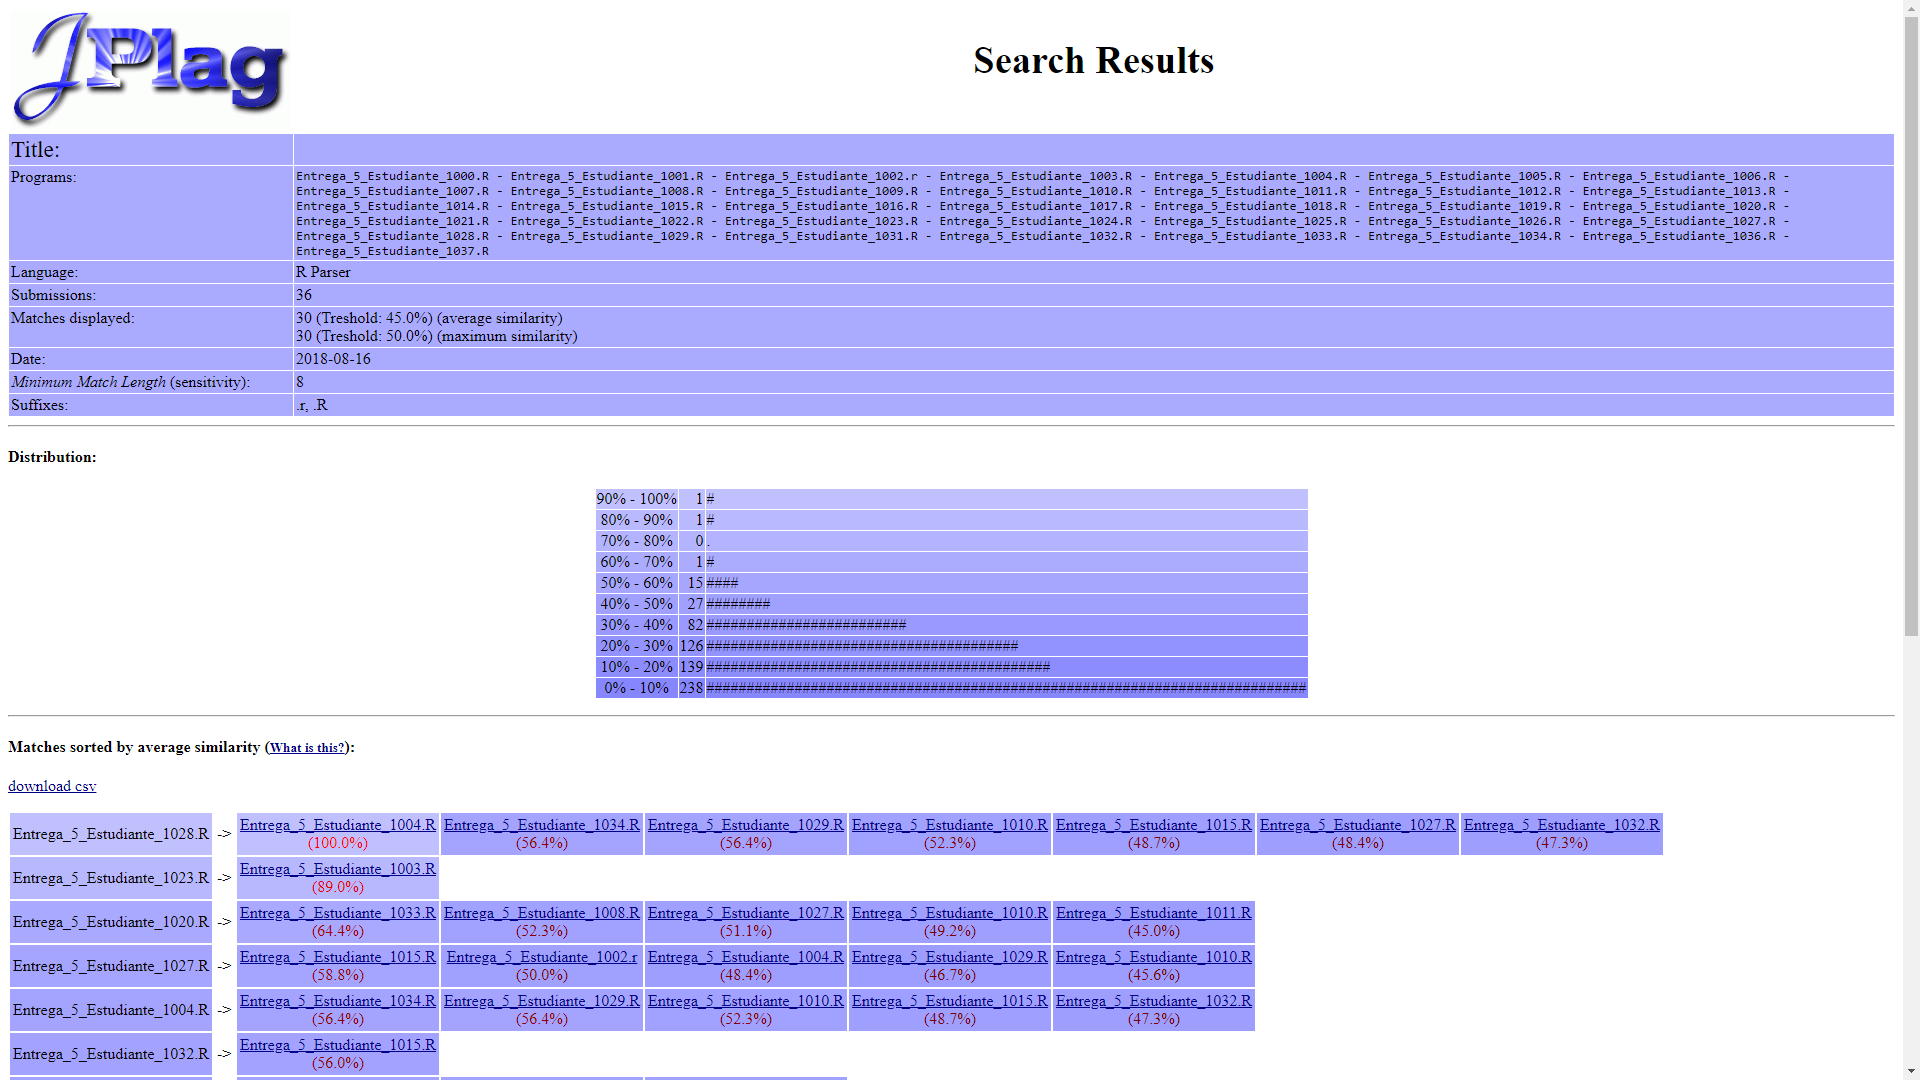
\includegraphics[ width=14cm, height=14cm]{imagenes/JPLAG_ejemplo_inicial.png}  %el parámetro scale permite agrandar o achicar la imagen. En el nombre de archivo puede especificar directorios
\caption{Ejemplo de página principal de resultados (JPLAG) } \label{fig:ej_JPLAG2}
\end{figure}

\begin{figure}[H] %con el [H] le obligamos a situar aquí la figura
\centering
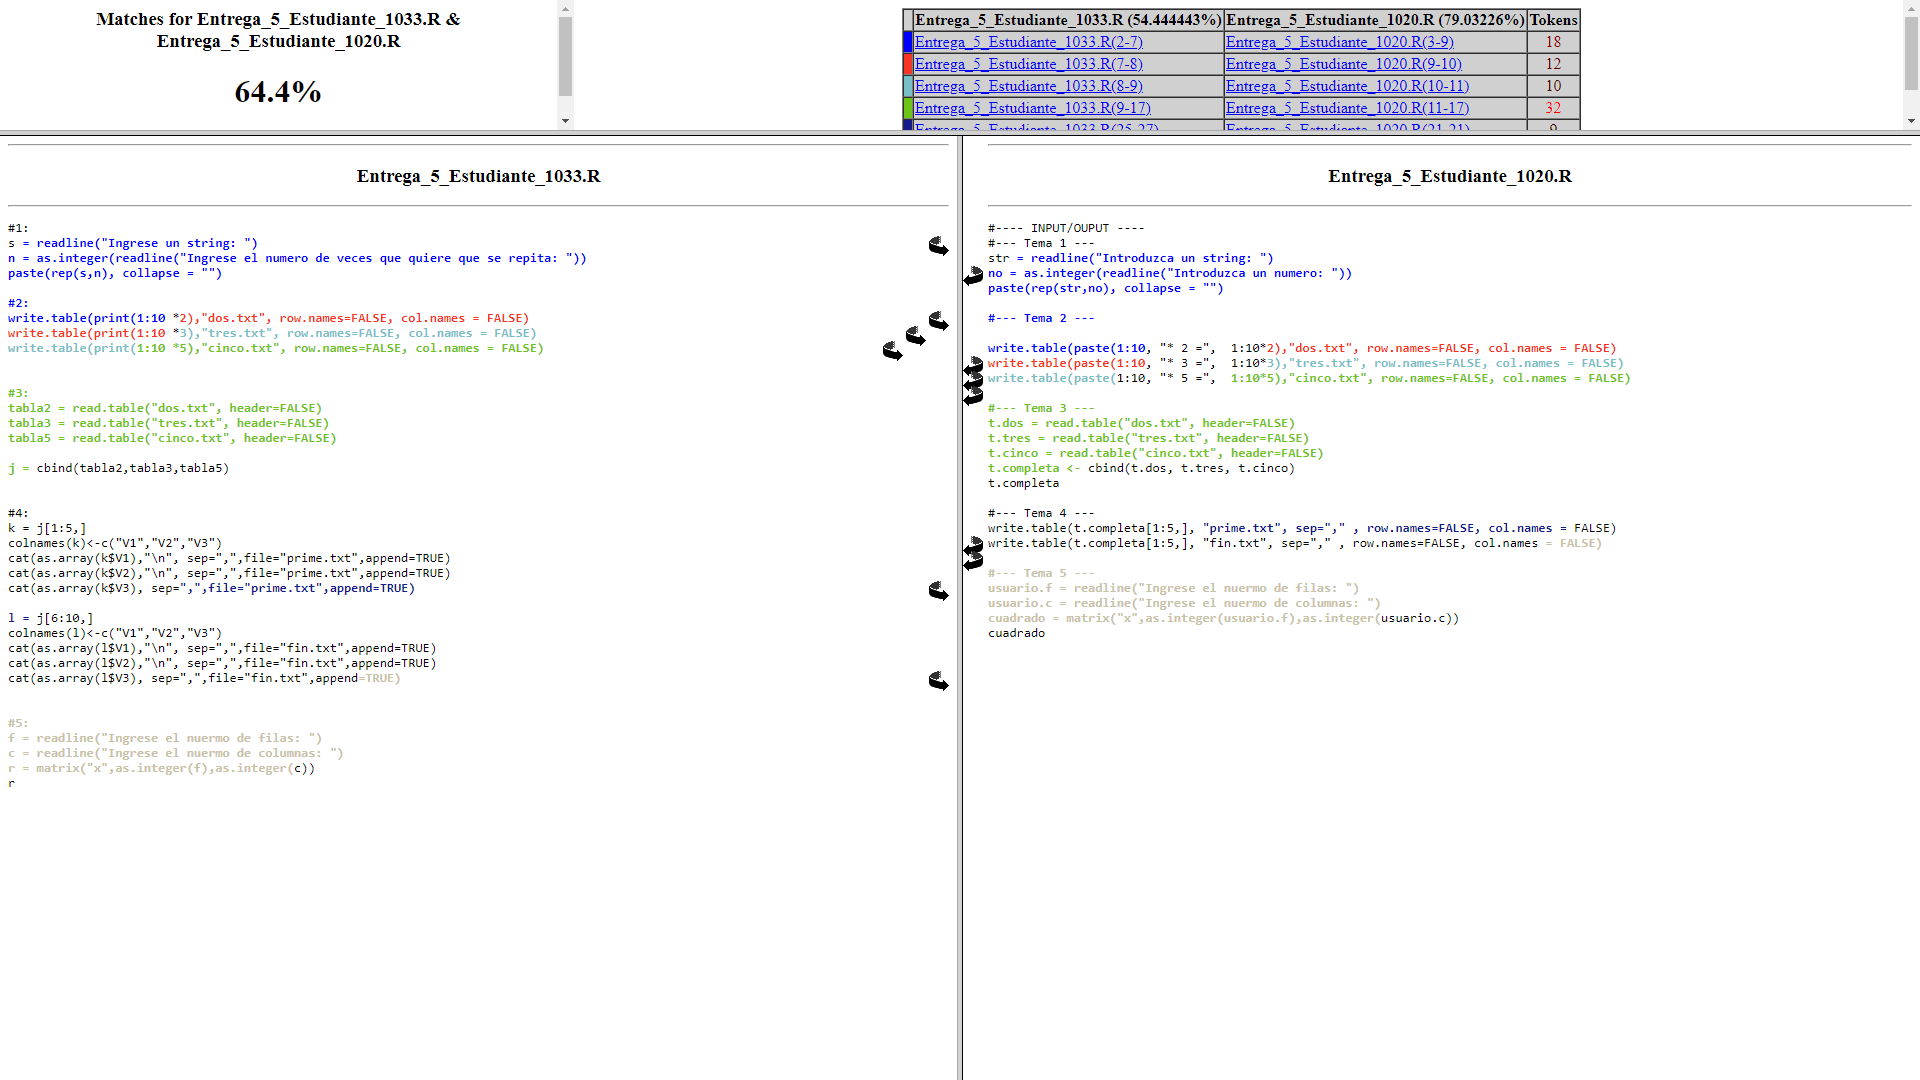
\includegraphics[ height=11cm, width=13cm]{imagenes/JPLAG_ejemplo_comparacion.png}  %el parámetro scale permite agrandar o achicar la imagen. En el nombre de archivo puede especificar directorios
\caption{Ejemplo de página de comparación de código de JPLAG} \label{fig:ej_JPLAG3}
\end{figure}

\subsection{Razones de su elección}
Dado que JPLAG es más fácilmente modificable, debido a que su código está disponible y no es necesario cambiar el algoritmo principal que usa para que funcione con otros lenguajes, (tan solo hay que crear un frontend) JPLAG ha sido la herramienta escogida para adaptar a R.




\chapter{Implementación}

\section{Estructura de nuestro frontend}
Se ha utilizado github y git para tener nuestra propia versión de JPLAG en nuestra cuenta de Github (https://github.com/AntonioJavierRP), gracias a esto podremos realizar los cambios que veamos necesarios en nuestra versión y mandar un pull request al repositorio original en \cite{jplag_github} por si el autor quiere incorporar el frontend que hemos creado para R a su versión.
\newline
Los cambios y las pruebas hechas en dicho código se han realizado en nuestra propia máquina local.
\newline
Nuestro frontend consta de la estructura de archivos que podemos ver en la Figura \ref{fig:ej_frontend} basada en los frontends ya existentes, especialmente en el de Java 1.7 y Python 3, ya que usan la misma herramienta que nosotros para crear el analizador sintáctico.

\begin{figure}[H] %con el [H] le obligamos a situar aquí la figura
\centering
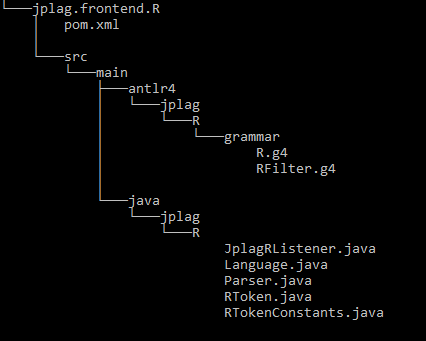
\includegraphics[scale=1]{imagenes/estructura_frontend.png}  %el parámetro scale permite agrandar o achicar la imagen. En el nombre de archivo puede especificar directorios
\caption{Árbol de archivos del frontend creado} \label{fig:ej_frontend}
\end{figure}

Como se puede apreciar, nuestro frontend consta de 8 archivos:
\begin{itemize}
\item \textbf{pom.xml}: archivo con la opciones de construcción y compilación de nuestro frontend en JPLAG.
\item \textbf{R.g4}: archivo de gramática que representa a R procesado por ANTLR4.
\item \textbf{RFilter.g4}: otro archivo de gramática que representa a R procesado por ANTLR4.
\item \textbf{JplagListener.java}: este archivo se encarga de seleccionar los tokens que mejor representan al lenguaje.
\item \textbf{Languaje.java}: en este archivo constan las características del lenguaje que JPLAG debe de saber antes de procesar los archivos enviados.
\item \textbf{Parser.java}: este archivo se encarga de extraer los tokens y de enviárselos a JPLAG.
\item \textbf{RToken.java y RTokenConstants.java}: en estos archivo especificamos los tokens importantes de R.
\end{itemize}
En los siguientes apartados se explica en más profundidad la función de cada uno de estos archivos.


\subsection{Apache Maven}

Para la construcción y gestión de JPLAG el autor original ha usado Maven.
\newline
Apache Maven es una herramienta de gestión y comprensión de proyectos software en Java \cite{maven_web}, es decir, es lo que se encarga de que se compilen todos los fuentes correctamente.
\newline
Maven permite la construcción de proyectos a través de archivos POM (project object model) y de un conjunto de plugins que tienen todos los proyectos que usan Maven (tiene que ser instalado previamente).
\newline
Un archivo pom.xml tiene una estructura básica similar a la que se muestra en el ejemplo a continuación en la Figura \ref{fig:ej_POM}.

\begin{figure}[H] %con el [H] le obligamos a situar aquí la figura
\centering
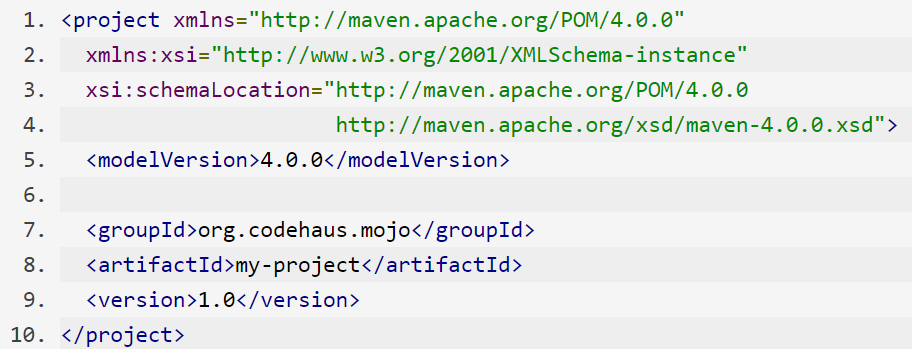
\includegraphics[scale=0.55]{imagenes/estructura_POM.png}  %el parámetro scale permite agrandar o achicar la imagen. En el nombre de archivo puede especificar directorios
\caption{Archivo ejemplo pom.xml} \label{fig:ej_POM}
\end{figure}

Para que nuestro frontend se tuviese en cuenta cuando se construye el proyecto se han tenido que modificar tres de los archivos pom.xml ya existentes en el proyecto añadiéndoles dependencias y módulos.
\newline
Así mismo se ha tenido también que crear nuestro propio archivo pom.xml dentro de nuestra carpeta del frontend como ya vimos en la Figura \ref{fig:ej_frontend}.

\section{Analizador utilizado}

Como ya mencionamos anteriormente, el frontend se encarga de reconocer las cadenas de tokens para que se les pueda aplicar el algoritmo. Para poder identificar estos tokens necesitamos un parser (analizador sintáctico).
\newline
En el resto de frontends los parser creados se han hecho usando JAVACC o ANTLR.
\newline
Estas son herramientas para la creación de analizadores de lenguajes basándose en gramáticas.
Para la creación de nuestro analizador sintáctico de R hemos escogido ANTLR4.



\subsection{ANTLR}
ANTLR (ANother Tool for Language Recognition) es un generador de analizadores sintácticos desarrollado por Terrence Parr \cite{antlr_libro}. 
\newline
Un analizador sintáctico procesa un trozo de texto y lo transforma en una estructura organizada, en un árbol de sintaxis. Este árbol representa la estructura lógica del contenido del código que ha procesado. Un ejemplo de tal árbol es el que vemos en la Figura \ref{fig:arbol_euclides} en el que se representa el código del algoritmo de Euclides.


\begin{figure}[] %con el [H] le obligamos a situar aquí la figura
\centering
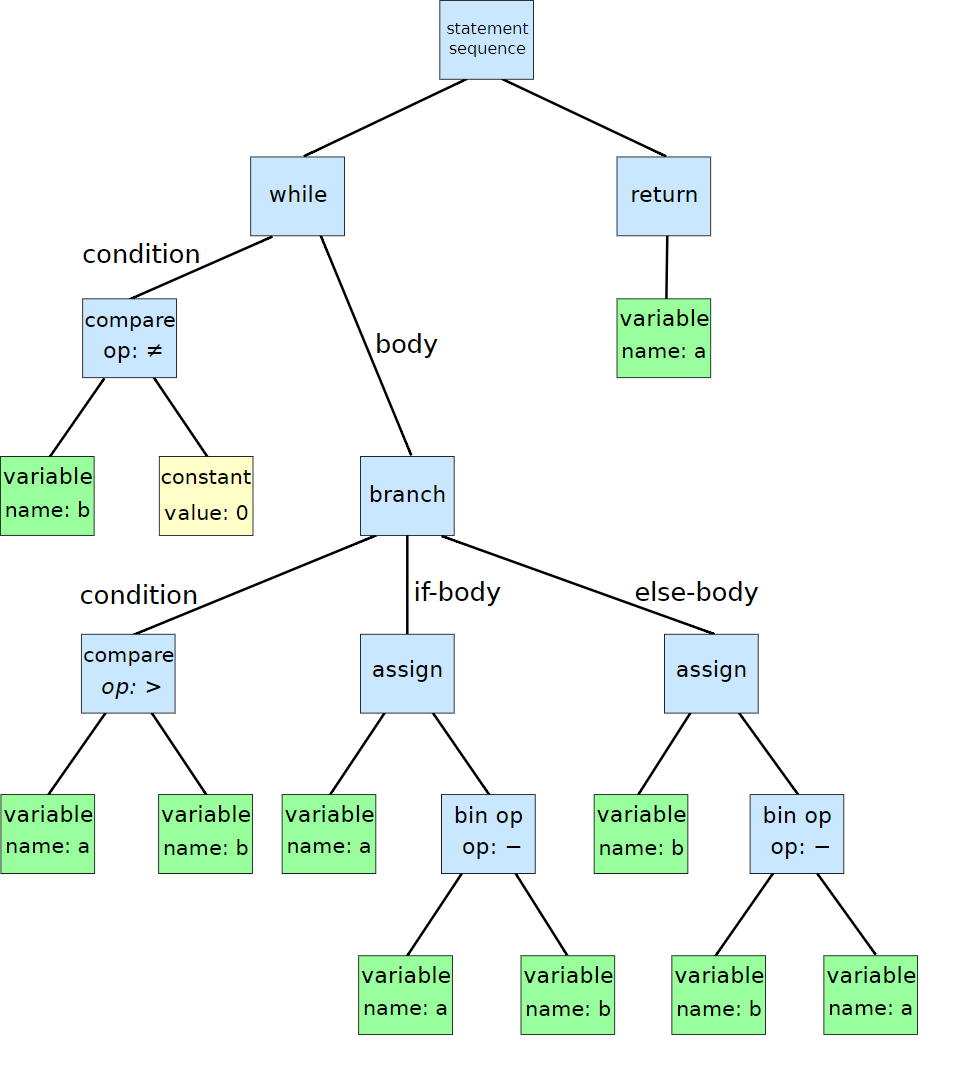
\includegraphics[scale=0.55]{imagenes/arbol.png}  %el parámetro scale permite agrandar o achicar la imagen. En el nombre de archivo puede especificar directorios
\caption{Árbol de sintaxis del algoritmo de Euclides.} \label{fig:arbol_euclides}
\end{figure}


Para obtener un árbol de sintaxis necesitaremos definir una gramática, invocar a ANTLR, para que genere un parser a partir de esta, y pasarle el código del que quieres obtener el árbol al parser.
\newline

ANTLR4 es la versión 4 de ANTLR y aporta numerosas nuevas funcionalidades que reducen la curva de aprendizaje necesaria para desarrollar la gramática de tu lenguaje. 
\newline
La característica más importante de esta versión es que acepta cualquier gramática que le hagas procesar a excepción de gramáticas con recursión indirecta por la izquierda (esto se da cuando una regla referencia a otra regla a la izquierda y esta segunda regla termina referenciando a la primera sin llegar a un símbolo terminal o token).
\newline
Los archivos que contienen la gramática tendrán que tener la extensión .g4, el nombre de la gramática como nombre del archivo y empezar con la línea de código : grammar $<nombre del archivo>$; . Aunque también puede comenzar siendo un parser grammar o lexer grammar si sólo vamos a definir reglas del analizador léxico o sintáctico. En nuestro caso el archivo se llama R.g4 y el archivo empieza con grammar R;.
\newline
El resto del archivo contendrá reglas del analizador léxico (lexer rules) y reglas del analizador sintáctico (parser rules).

\bigskip

Las ''lexer rules'' son las definiciones de los tokens básicos que conforman el lenguaje y siguen la sintaxis de las reglas sintácticas. Las reglas del analizador léxico se escriben en mayúscula y al final del archivo, en Figura \ref{fig:lexer_rules} podemos ver un ejemplo de estas reglas.

\begin{figure}[] %con el [H] le obligamos a situar aquí la figura
\centering
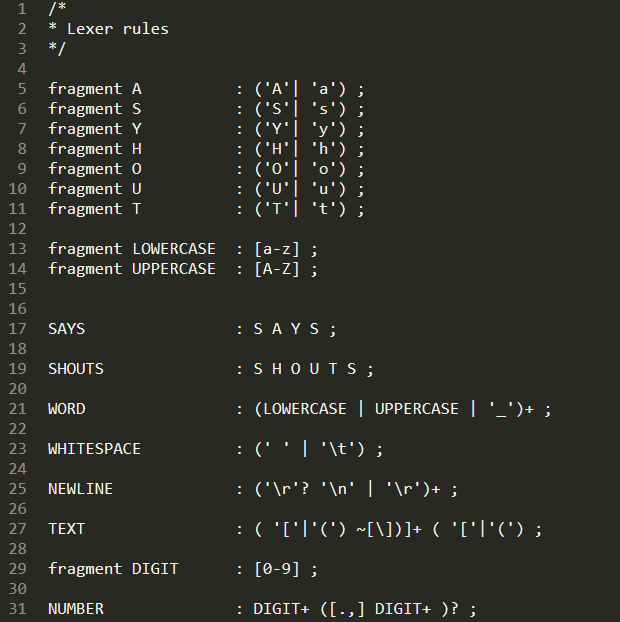
\includegraphics[scale=0.55]{imagenes/lexer_rules.png}  %el parámetro scale permite agrandar o achicar la imagen. En el nombre de archivo puede especificar directorios
\caption{Ejemplo de lexer rules.} \label{fig:lexer_rules}
\end{figure}

\bigskip

Las ''parser rules'' son la reglas que muestran las combinaciones posibles de los tokens básicos (definidos en las lexer rules) en el lenguaje.
\newline
Tenemos una primera regla (en el ejemplo que mostramos es 'chat') que genera el resto de reglas.
Estas reglas se escriben en minúsculas y se deben de poner antes que las reglas del analizador léxico.
\newline
Podemos ver un ejemplo de estas en la Figura \ref{fig:parser_rules}.

\begin{figure}[] %con el [H] le obligamos a situar aquí la figura
\centering
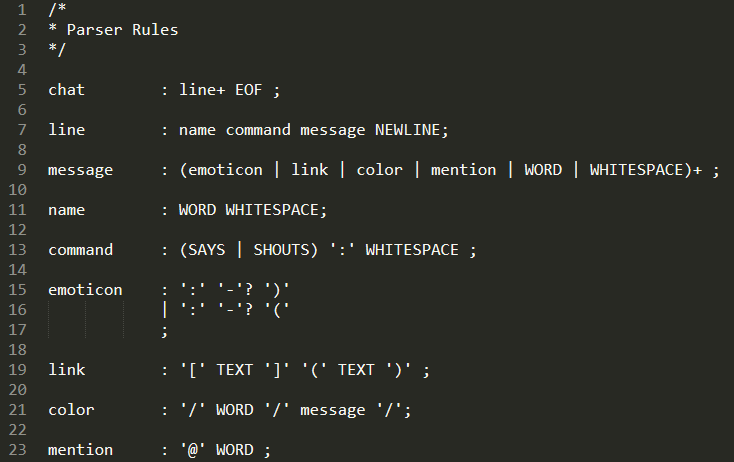
\includegraphics[scale=0.55]{imagenes/parser_rules.png}  %el parámetro scale permite agrandar o achicar la imagen. En el nombre de archivo puede especificar directorios
\caption{Ejemplo de parser rules.} \label{fig:parser_rules}
\end{figure}


\section{Adaptación del parser a JPLAG}

La gramática que hemos usado se encuentra en el archivo R.g4 junto con RFilter.g4.
Nuestra gramática está basada en una ya existente para R en ANTLR4 encontrada en \cite{repositorio_gramatica}. Hemos añadido una gran cantidad de reglas del análisis sintáctico nuevas en el archivo R.g4 para poder quedarnos con los tokens más representativos del lenguaje ya que necesitamos que los tokens que estamos agrupando aparezcan agrupados como parser rule, como por ejemplo, en el caso de los tokens para el flujo de control ''if''. Hemos creado la siguiente regla:

\begin{center}
\begin{lstlisting}
if_statement :  'if' '(' expr ')' expr | 'if' '(' expr ')' expr 'else' expr ;
\end{lstlisting}
\end{center}

Esta regla la hemos creado de forma separada para que después en el Listener(que crea ANTLR4 al procesar la gramática) podamos reconocerla. Este Listener contiene métodos que se llaman cuando se entra o sale de cada regla del analizador sintáctico.
\newline
Es por eso que en archivo JplagRListener.java lo que hacemos es implementar ese Listener (ya que se trata de una interfaz) para que cada vez que se llame a un método de una regla asociada a un token que queramos se añada a la cadena de tokens del archivo que estamos procesando.
\newline
\newline
El archivo RFilter.g4 tan solo contiene reglas para eliminar saltos de linea que en realidad son espacios en blanco así que no lo hemos modificado.
\newline
Las funciones que se encargan de cargar los archivos, llamar al analizador sintáctico para obtener los tokens de estos y mandar los tokens encontrados a JPLAG están en el archivo parser.java.
\newline
En languaje.java especificamos las extensiones válidas que requiere que tengan los archivos del lenguaje, el nombre del parser y el número mínimo de emparejamientos seguidos de tokens que deben hacerse para poder marcarlo como emparejamiento (tal y como explicamos en el apartado del algoritmo). El resto de métodos especifican opciones que no vamos a variar respecto de los otros frontends.
\newline
Por último, en RTokenConstants.java especificamos el nombre de los tokens más importantes del lenguaje en una interfaz llamada RTokenConstants, mientras que en RToken.java implementamos esta interfaz añadiéndole un método que devuelve los tokens pasados a string.

\bigskip

Una vez hecha toda esta implementación, hemos terminado la creación del frontend, realizamos entonces las pruebas necesarias para comprobar si la lista inicial de tokens seleccionados de R representa suficientemente bien al lenguaje. 
\newline 
 Terminamos realizando modificaciones y seleccionamos más tokens basándonos en los seleccionados en el resto de frontends y en la página de referencia del lenguaje R \cite{R_language_definition}.


%
\chapter{Ejecución y Pruebas}


\subsubsection{Instrucciones de uso y ejecución}

En los siguiente apartados mostramos los pasos a seguir para la obtención de resultados en MOSS y en JPLAG.

\section{Ejecución en MOSS}

Siguiendo las instrucciones en \cite{Moss_web} y en \cite{instrucciones_moss} sabemos que, para poder comunicarnos en el servidor de MOSS y mandarle los archivos, necesitaremos un script en Perl.
\newline
Para obtener este script enviamos un mensaje por correo electrónico a 
\newline 
moss@moss.stanford.edu con lo siguiente en el cuerpo del mensaje:

\begin{center}
registeruser
\\mail usuario@dominio
\end{center}

En nuestro caso pondremos antoniojrp@correo.ugr.es en la parte de usuario@dominio.
\newline
Unos cinco minutos después del envío de este mensaje recibiremos una respuesta automática del servidor en nuestro correo con el script que necesitamos y con instrucciones de su uso.
En el script se detalla que podemos compartir este script con otros profesores de programación pero que por favor no lo compartamos en un sitio de acceso público (''Feel free to share this script with other instructors of programming classes, but please do not place the script in a publicly accessible place.''), por esta razón no mostramos el contenido completo del script en esta memoria.

\bigskip
Ahora que tenemos el script, lo colocamos en el directorio donde tenemos los archivos o las carpetas de los archivos que queremos comparar, para mayor comodidad a la hora de escribir las rutas de los archivos al llamar al script.
\newline
Nos situamos con la terminal (este script funciona en Unix, en caso estar en Windows se tendrá que usar Cygwin) en el directorio donde está el script y ejecutamos los siguientes comandos:

\bigskip

Para modo Matlab:
\begin{center}
\begin{lstlisting}[language=bash]
$ ./moss -l matlab -c "Entrega X" "Entrega X"/*.r "Entrega X"/*.R
\end{lstlisting}
\end{center}


Para modo texto plano:
\begin{center}
\begin{lstlisting}[language=bash]
$ ./moss -l ascii -c "Entrega X" "Entrega X"/*.r "Entrega X"/*.R
\end{lstlisting}
\end{center}

Entrega X es la entrega de alumnos que queremos evaluar actualmente, ya que en nuestro caso hay un total de 7 entregas diferentes ( siete trabajos diferentes con más de 30 archivos de ejercicios de alumnos en R en cada uno), y hemos nombrado el directorio donde se encuentran cada una de las entregas ''Entrega 1'', ''Entrega 2'', ''Entrega 3'', etc hasta siete entregas.

\bigskip

\subsubsection{Explicación de opciones:}

Con la opción -l especificamos el lenguaje en el que (supuestamente) están los archivos para que MOSS lo tenga en cuenta en su algoritmo. En nuestro caso hemos decidido realizar las pruebas como si los archivos estuvieran escritos en texto plano y en Matlab (dado que es el más similar a R de todas las posibles opciones). Si esta opción se deja vacía, MOSS supondrá que los archivos están en C.

\bigskip

Con la opción -c le asocia un nombre a los resultados que se generan. En nuestro caso le asociamos el número de la entrega.

\bigskip

Entre las opciones que no hemos especificado tenemos:

\begin{itemize}
\item -m: Especifica el número máximo de veces que un mismo fragmento de código tiene que aparecer para que se ignore en los emparejamientos. Por defecto esta opción tiene el valor 10.
\item -d: Especifica que los archivos a evaluar se agrupan por directorio y no por archivos individuales, es decir, cada alumno es un directorio completo lleno de archivos y se compara entre directorios.
\item -b: Nos permite especificar un archivo base. El código que tengan en común el resto de archivos con el archivo base no se tendrá en cuenta en los emparejamientos.
\end{itemize}

Al ejecutar estos comandos, le enviamos los archivos al servidor y obtenemos un enlace como el siguiente:
\begin{center}
http://moss.stanford.edu/results/169343157
\end{center}
Es posible que en el momento que se lea esto el enlace de ejemplo no exista ya que el servidor borra los resultados 15 días después de generarlos.
\newline
En nuestro caso han tardado de media un minuto en generarse, variando en función del tamaño de los archivos de la entrega (treinta segundos para la entrega más corta y un minuto y cuarenta segundos para la más larga). 
\newline
Al acceder a este enlace podemos ver en nuestro navegador una página principal con los resultados, en el caso por ejemplo de la Entrega 2, hemos obtenido la página de resultados de la Figura \ref{fig:entrega2_MOSS_1}.
\newline
La página muestra la fecha en la que fue generada, las opciones de ejecución elegidas a la hora de ejecutar el script y la etiqueta que le asociamos con la opción -c.
\newline
Seguido de esto tenemos seis links de ayuda con las bases de cómo interpretar los resultados, contacto y créditos.
\newline
El resto de la página contiene una tabla de pares de archivos con código similar, ordenado por la cantidad de código en común entre estos.
\newline
Al final del nombre de cada archivo está el porcentaje del código de ese archivo que se considera coincidente con el del otro en su misma línea.
\newline
Por último cabe mencionar que la columna ''Lines Matched'' contiene el número aproximado de lineas de código emparejadas entre los archivos de la fila.


\begin{figure}[] %con el [H] le obligamos a situar aquí la figura
\centering
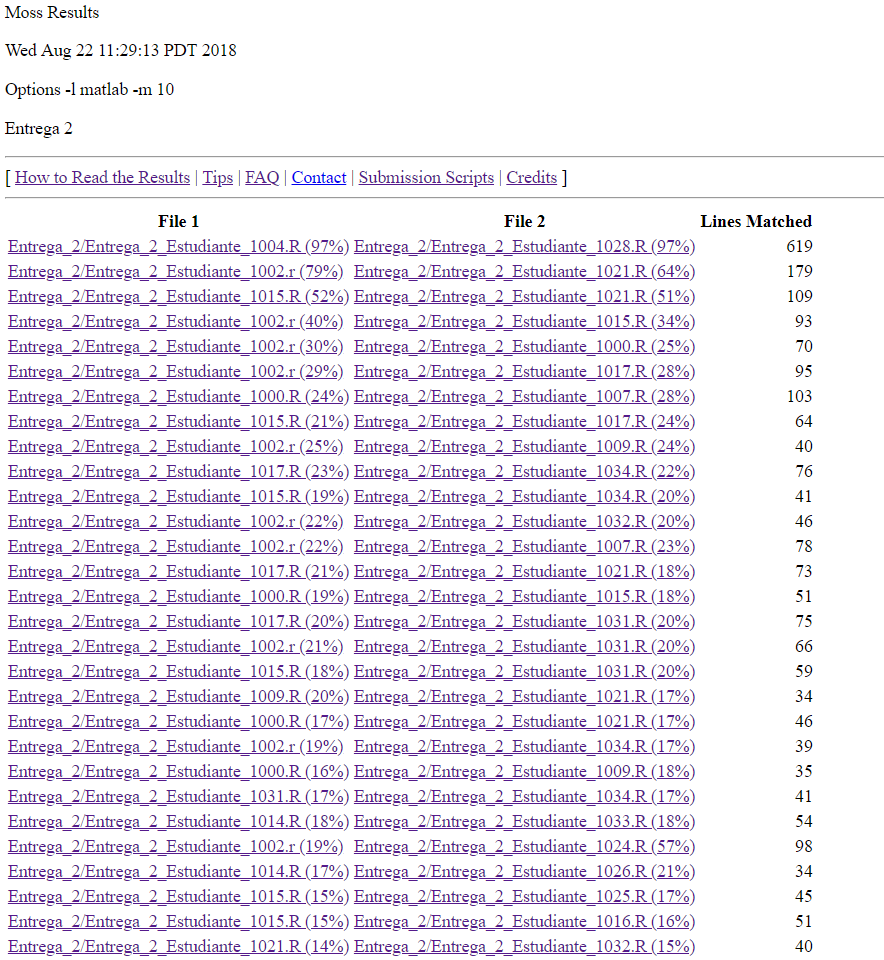
\includegraphics[ width=13cm, height=15cm]{imagenes/entrega2_MOSS_main.png}  %el parámetro scale permite agrandar o achicar la imagen. En el nombre de archivo puede especificar directorios
\caption{Página principal de resultados de la segunda entrega con matlab como opción (MOSS) } \label{fig:entrega2_MOSS_1}
\end{figure}

La mejor estrategia para interpretar estos resultados es empezar evaluando los archivos con mayor porcentaje coincidente e ir bajando en la lista hasta que los archivos que estemos comprobando estén llenos de emparejamientos que sean falsos positivos.

\bigskip

Por cada par de archivos emparejados hay una página con información sobre los fragmentos que coinciden. Esta página esta estructurada en tres marcos: uno con una tabla con todos los fragmentos coincidentes (Figura \ref{fig:entrega2_MOSS_2}), y los otros dos con el código de cáda archivo(Figura \ref{fig:entrega2_MOSS_3}).


\begin{figure}[] %con el [H] le obligamos a situar aquí la figura
\centering
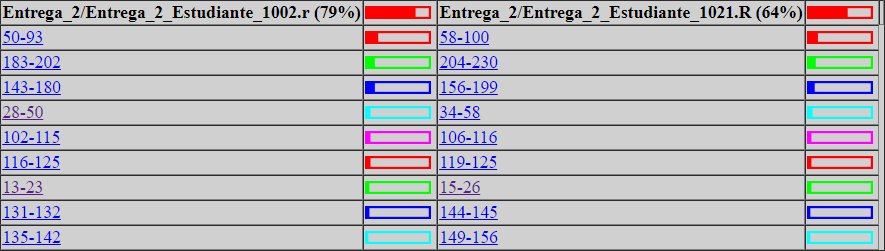
\includegraphics[scale=0.5]{imagenes/entrega2_MOSS_tabla.png}  %el parámetro scale permite agrandar o achicar la imagen. En el nombre de archivo puede especificar directorios
\caption{Tabla comparativa entre dos estudiantes en la segunda entrega con matlab como opción (MOSS)} \label{fig:entrega2_MOSS_2}
\end{figure}


\begin{figure}[] %con el [H] le obligamos a situar aquí la figura
\centering
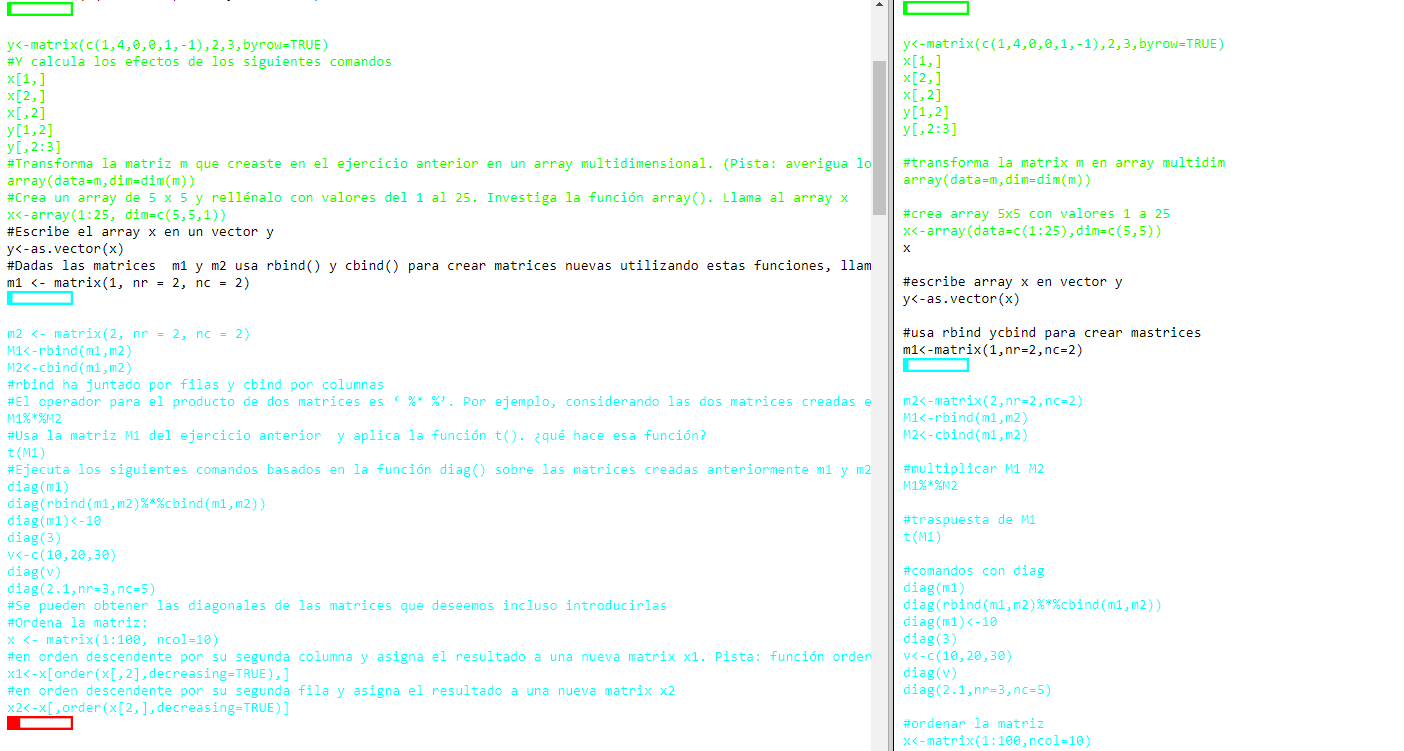
\includegraphics[width=14cm, height=10cm]{imagenes/entrega2_MOSS_comp.png}  %el parámetro scale permite agrandar o achicar la imagen. En el nombre de archivo puede especificar directorios
\caption{Parte comparativa del código fuente de dos estudiantes en la segunda entrega con matlab como opción (MOSS)} \label{fig:entrega2_MOSS_3}
\end{figure}


En la tabla de Figura \ref{fig:entrega2_MOSS_2} se muestra un rango con el número de líneas de cada archivo donde se considera que ha habido copia, junto con un ''termómetro'' para mostrar gráficamente cómo de grande es este fragmento en comparación con el archivo completo.
Estos ''termómetros'' así mismo son links que te situan en la parte del código al que se refieren en los otros dos marcos (Figura \ref{fig:entrega2_MOSS_3}).

\bigskip
\section{Ejecución en JPLAG}

Para usar JPLAG tendremos que descargar el código fuente completo de \cite{jplag_github}. Para usar nuestra versión con nuestro frontend de R podemos descargar el código de https://github.com/AntonioJavierRP/jplag.
\newline
Una vez hecho esto nos situamos con nuestra terminal en la carpeta principal, es decir, la que contiene todos los frontends. Para generar los ejecutables de cada frontend ejecutaremos la orden:
\begin{center}
\begin{lstlisting}[language=bash]
$ mvn clean generate-sources package
\end{lstlisting}
\end{center}
En caso de querer generar un único ejecutable usaremos la siguiente orden dentro de la carpeta jplag:
\begin{center}
\begin{lstlisting}[language=bash]
$ mvn clean generate-sources assembly:assembly
\end{lstlisting}
\end{center}
Para ejecutar cualquiera de las dos últimas ordenes es necesario tener instalado Apache Maven, las instrucciones de su instalación se encuentran en \cite{instalacion_maven}
\newline
Los ejecutables creados estarán en sus respectivas carpetas ''target'', en el caso de tener un único ejecutable este estará en jplag/target.
\newline

\subsection{Obtención de resultados}

En nuestro caso hemos llamado a JPLAG con las siguientes opciones (situándonos en jplag/target):

\begin{center}
\begin{lstlisting}[language=bash]
$ java -jar jplag-2.11.9-SNAPSHOT-jar-with-dependencies.jar -l R -r ../resultados/Entrega_X/ -s <ruta_directorio_entrega_X>
\end{lstlisting}
\end{center}

Se ha ejecutado esta orden para siete entregas distintas, con unos 30 archivos por entrega, dos veces, una para R y otra para texto plano.
\newline
Como se puede apreciar se ha usado la opción -l para especificar el lenguaje, -r para especificar donde guardar los resultados y -s para especificar la ruta donde se encuentran todos los archivos que se quieren evaluar.
Podemos visualizar el resto de opciones disponibles con su descripción ejecutando el .jar sin opciones:
\begin{center}
\begin{lstlisting}[language=bash]
$ java -jar jplag-2.11.9-SNAPSHOT-jar-with-dependencies.jar
\end{lstlisting}
\end{center}

Los resultados serán visualizables en el navegador, podemos abrir el archivo index.html para situarnos en la página principal de análisis de los resultados (Figuras \ref{fig:entrega2_JPLAG_1} y \ref{fig:entrega2_JPLAG_2}).
La interpretacion de estos resultados es muy similar a la que explicamos en apartados anteriores con MOSS, ya que su interfaz es muy similar.
\newline
A continuación explicamos cómo interpretar los elementos de la página principal de JPLAG.
\begin{figure}[t] %con el [H] le obligamos a situar aquí la figura
\centering
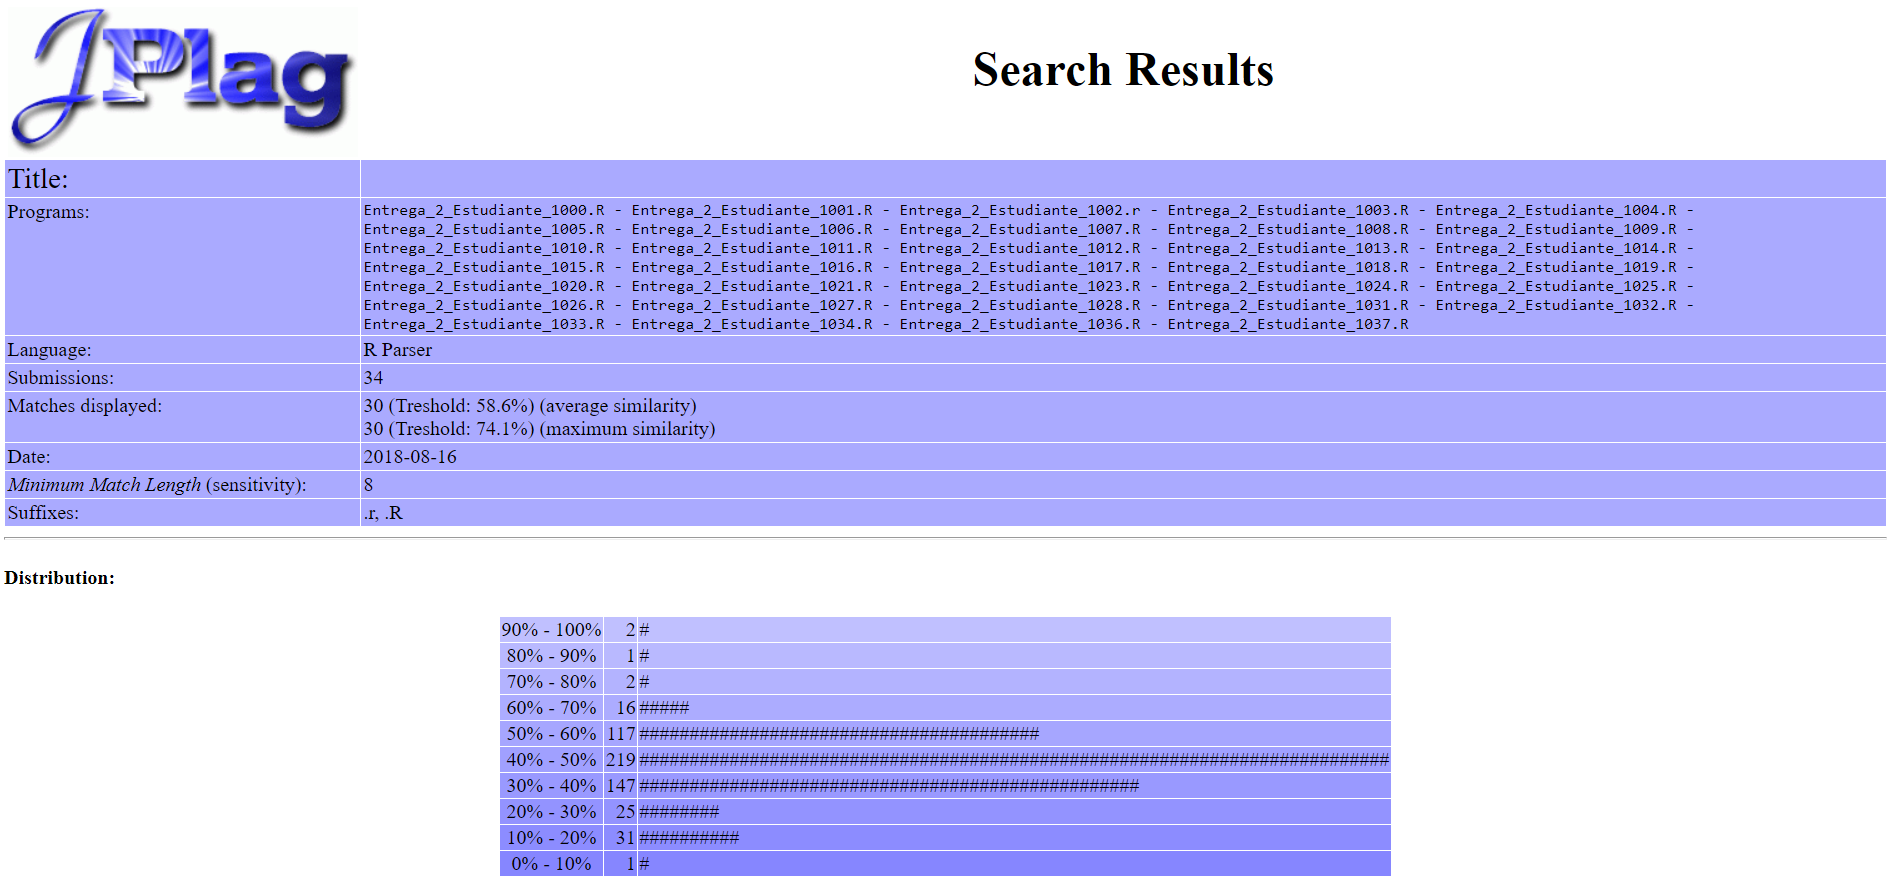
\includegraphics[width=14cm, height=9cm]{imagenes/entrega2_JPLAG_1.png}  %el parámetro scale permite agrandar o achicar la imagen. En el nombre de archivo puede especificar directorios
\caption{Página principal de los resultados de la Entrega 2 (JPLAG) parte 1} \label{fig:entrega2_JPLAG_1}
\end{figure}

\begin{figure}[t] %con el [H] le obligamos a situar aquí la figura
\centering
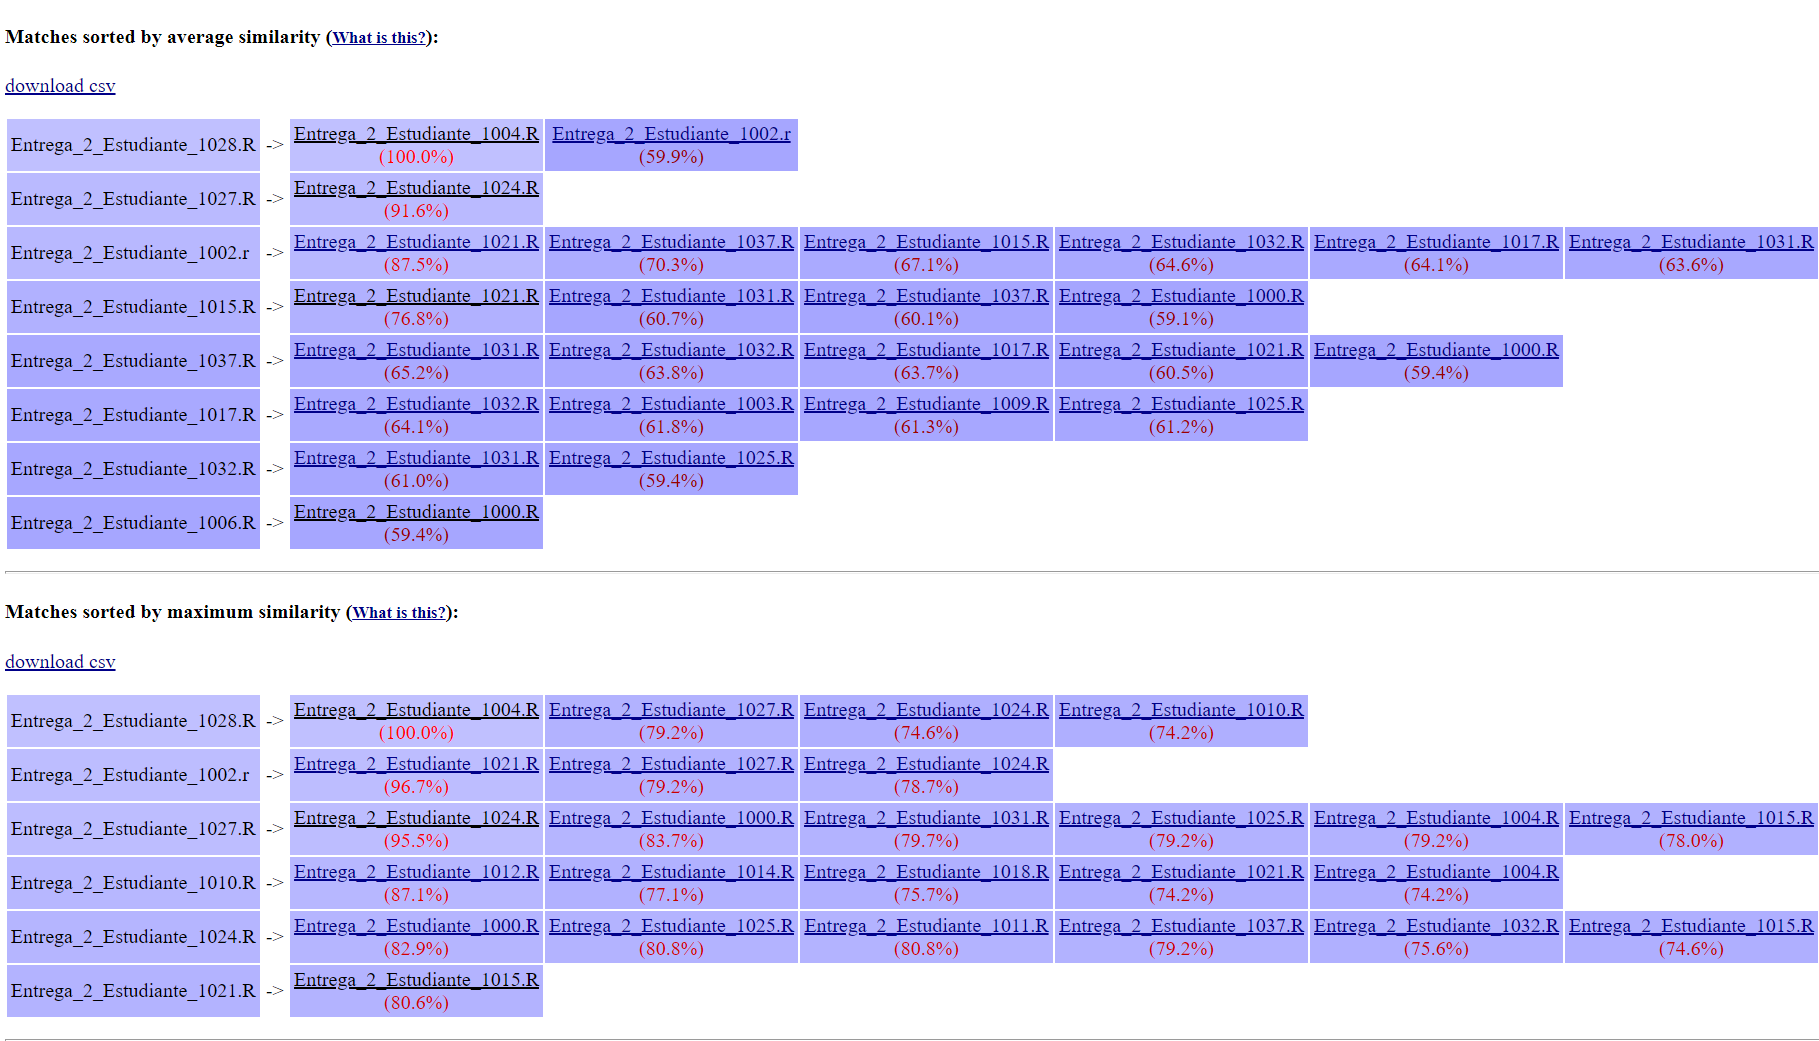
\includegraphics[width=14cm, height=9cm]{imagenes/entrega2_JPLAG_2.png}  %el parámetro scale permite agrandar o achicar la imagen. En el nombre de archivo puede especificar directorios
\caption{Página principal de los resultados de la Entrega 2 (JPLAG) parte 2} \label{fig:entrega2_JPLAG_2}
\end{figure}
La Figura \ref{fig:entrega2_JPLAG_1} contiene la parte de arriba de la página de resultados de la segunda entrega de los alumnos obtenida por nuestro frontend de R.
Se lista en una tabla el nombre de los programas que se han detectado, el idioma del parser usado, el número de archivos totales, el número de archivos emparejados que se muestran, la fecha en la que se obtuvieron los resultados, el número mínimo de tokens iguales que tiene que haber para que se considere un emparejamiento y las extensiones de los archivos procesados.
\newline
Seguido de esto, JPLAG muestra un histograma de los valores de similaridad encontrados en todos los pares de programas.
\newline
Podemos usar este histograma para identificar los casos que son plagio obvio y los que no tienen nada en común.
\newline
Los pares que se encuentran entre estos dos lados del espectro se encuentran a continuación en la parte de abajo de la página en Figura \ref{fig:entrega2_JPLAG_2}.
\newline
Se muestran ordenados en base a dos criterios, basándose en la cobertura entre programas (es decir, cuánto de un programa se ha usado en otro):
\begin{itemize}
\item Similaridad Media: media entre las coberturas de ambos programas entre si. Emparejamientos con una alta cobertura indican pares muy similares.
\item Similaridad Máxima: el máximo entre las dos coberturas. Esta medida es útil para encontrar los casos en los que ha habido plagio y se ha añadido código extra para ''rellenar'' y que los archivos tengan tamaños muy diferentes.
\end{itemize}

Haciendo click en el nombre de alguno de estos archivos iremos a la página comparativa de código entre estos.
\newline
En la parte superior de la página (Figura \ref{fig:entrega2_JPLAG_3}) tenemos a la izquierda el nombre de los archivos que se comparan, su porcentaje de similaridad y dos hiperlinks uno para volver a la página principal y otro de ayuda. A la derecha de esta página se muestra una tabla similar a la que teníamos en MOSS, en la que también se listan los trozos de código donde se han encontrado cadenas de tokens idénticas. Por cada par de trozos de código se especifica el número de tokens en común que se han encontrado seguidos y el color que se le ha asignado para que su visualización sea más facil en la parte de abajo de esta misma página (Figura \ref{fig:entrega2_JPLAG_4}).
\newline
En esta parte cada pasaje encontrado tiene una especie de flecha al principio, al pinchar sobre esta se alinea la otra parte del código del otro programa para que se puedan ver lado a lado los trozos de código con el mismo color.
Si una parte del código no coincide con la del otro programa esta se mostrará en color negro.


\begin{figure}[H] %con el [H] le obligamos a situar aquí la figura
\centering
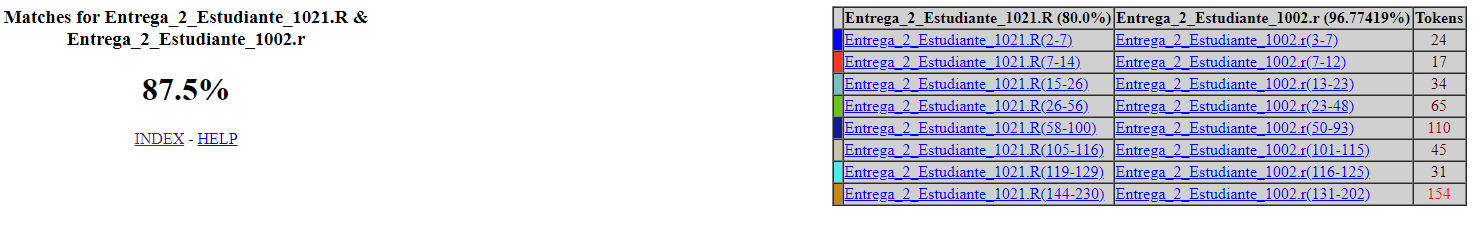
\includegraphics[scale=0.3]{imagenes/entrega2_JPLAG_3.png}  %el parámetro scale permite agrandar o achicar la imagen. En el nombre de archivo puede especificar directorios
\caption{Página de comparación de código entre dos archivos en JPLAG (parte de arriba)} \label{fig:entrega2_JPLAG_3}
\end{figure}


\begin{figure}[H] %con el [H] le obligamos a situar aquí la figura
\centering
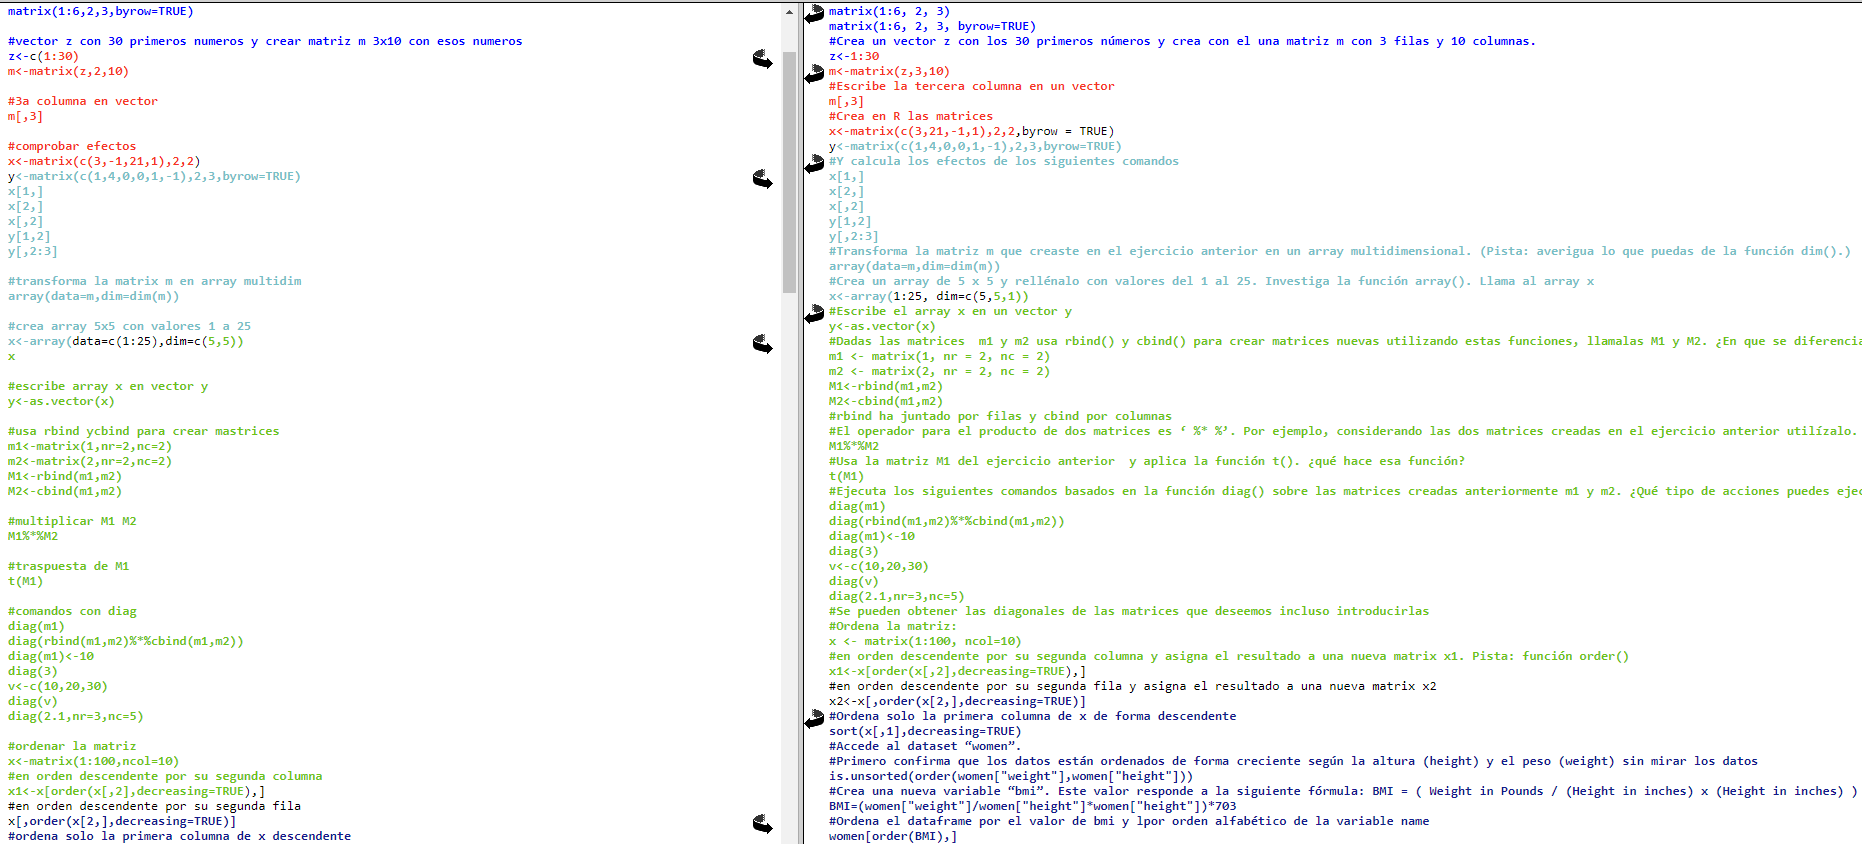
\includegraphics[width=14cm, height=9cm]{imagenes/entrega2_JPLAG_4.png}  %el parámetro scale permite agrandar o achicar la imagen. En el nombre de archivo puede especificar directorios
\caption{Página de comparación de código entre dos archivos en JPLAG (parte de abajo)} \label{fig:entrega2_JPLAG_4}
\end{figure}

\section{Pruebas}

Para comprobar que el frontend que hemos creado facilita la detección de plagio entre archivos en R, se ha hecho un estudio de las diferencias entre los resultados obtenidos con nuestra versión de JPLAG usando el frontend de R y los resultados que se podían obtener usando otros medios ya existentes.
\newline
Los archivos en R usados para realizar este estudio han sido las entregas de los alumnos de la asignatura ''Introducción a la programación para ciencia de datos'' del Master de ciencia de datos de la Universidad de Granada.
\newline
Cada entrega consiste en ejercicios sobre diferentes aspectos de R, empezando por una introducción con ejercicios simples y añadiendo nuevos conceptos y estructuras de R con cada nueva entrega.
\newline
Son un total de 7 entregas:
\begin{itemize}
\item \textbf{Entrega 1.} Introducción a R y ejercicios de vectores. 36 programas enviados(cada programa es un archivo de un único alumno).
\item \textbf{Entrega 2.} Ejercicios de matrices, arrays y factores. 34 programas enviados.
\item \textbf{Entrega 3.} Ejercicios de manipulación de strings. 36 programas enviados.
\item \textbf{Entrega 4.} Ejercicios de dataframes y listas. 33 programas enviados.
\item \textbf{Entrega 5.} Ejercicios de entrada y salida. 36 programas enviados.
\item \textbf{Entrega 6.} Ejercicios de Funciones. 36 programas enviados.
\item \textbf{Entrega 7.} Ejercicios de estructuras de programación en R. 36 programas enviados.
\end{itemize}
Los ejercicios de los alumnos se han convertido a archivos .R (ya que en algunos archivos estaban en .pdf, .docx, .rmd,...) para que JPLAG los pueda procesar y han sido ademas anonimizados asignándosele a cada alumno un ID. Hay 38 alumnos en total.
\newline
Cada una de estas entregas ha sido procesada en JPLAG con nuestro frontend, con el frontend de texto plano y en MOSS en modo Matlab y texto plano.

Se han analizado los resultados en base a las entregas:
\subsection{Análisis de resultados}

Se han analizado los resultados en base a las peculiaridades de cada entrega, ya que estas se dividen en diferentes aspectos del lenguaje, lo cual es idóneo para observar la precisión de la detección de plagio en ejercicios de áreas totalmente distintas.

\bigskip


La primera entrega consiste en una serie de ejercicios de introducción a R, para que el alumno aprenda cómo generar secuencias de números, usar vectores y a usar las llamadas más comunes que se usan en R.
\newline
Por norma general los alumnos han necesitado aproximadamente cien líneas de código para completar estos ejercicios, aunque los programas tienen más de doscientas en total debido a comentarios con aclaraciones sobre el código y con los enunciados de los ejercicios.
\newline
Los resultados obtenidos en esta entrega con JPLAG se pueden ver plasmados en dos histogramas en Figura \ref{fig:histograma1} donde se muestran los valores de similaridad media para todos los pares posibles de programas (en esta entrega al ser 36 programas habrá 630 emparejamientos diferentes).


\begin{figure}[H] %con el [H] le obligamos a situar aquí la figura
\centering
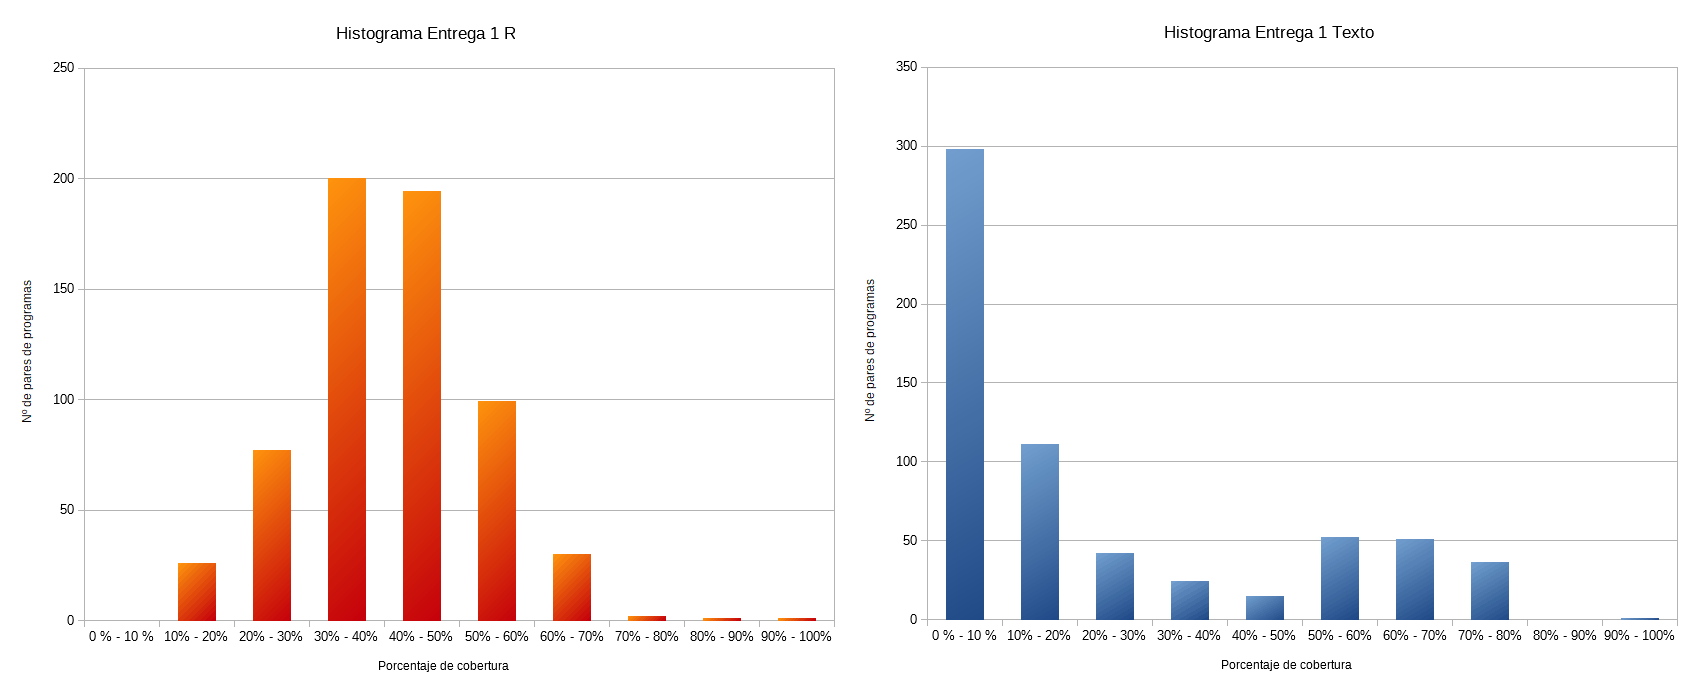
\includegraphics[width=15cm, height=7cm]{imagenes/histograma1.png}  %el parámetro scale permite agrandar o achicar la imagen. En el nombre de archivo puede especificar directorios
\caption{Histogramas de valores de similaridad entre todos los pares de programas de la primera entrega.} \label{fig:histograma1}
\end{figure}



Para evitar mostrar este caso repetidas veces con cada gráfica que se muestre, se ha de mencionar que en todas las entregas hechas menos en la séptima, los estudiantes con id 1004 y 1028 se han copiado al 100\%, es decir, han entregado programas iguales.
\newline
\bigskip

Como era de esperar, el frontend de JPLAG de texto plano, correspondiente al histograma de la derecha, sólo detecta plagio en caso de que se haya hecho una copia literal del código, es decir, que sea exáctamente el mismo con las mismas palabras. Por esta razón la mayor parte de los pares de programas tienen un índice de cobertura (o similaridad) muy bajo. Existen algunos casos con un índice alto, pero esto se debe a similaridad en los comentarios, ya que algunos alumnos han escrito en los comentarios del programa el enunciado de los ejercicios o explicaciones similares.
\newline
En el caso de nuestro frontend de R (histograma a la izquierda), se detectan una gran cantidad de pares con un índice de cobertura superior al treinta porciento, esto se debe a que los ejercicios de esta entrega son muy concretos y no hay muchas formas de hacerlos por lo que es normal que los alumnos hayan usado estructuras muy similares que al fin y al cabo están formadas por los mismos tokens.
\newline
Los pares con un índice superior al 70 porciento son casos casi seguros de plagio ya que es altamente improbable que dos alumnos tengan más de un setenta porciento de su código estructuralmente igual en 100 líneas de código sin haberse copiado.
\newline
En las gráficas de Figura \ref{fig:TOP10_1} podemos ver una representación de los resultados obtenidos en MOSS.
\newline 
En estas gráficas figuran los índices de similaridad de los 10 pares de programas más ''parecidos'' de la primera entrega. 


\begin{figure}[H] %con el [H] le obligamos a situar aquí la figura
\centering
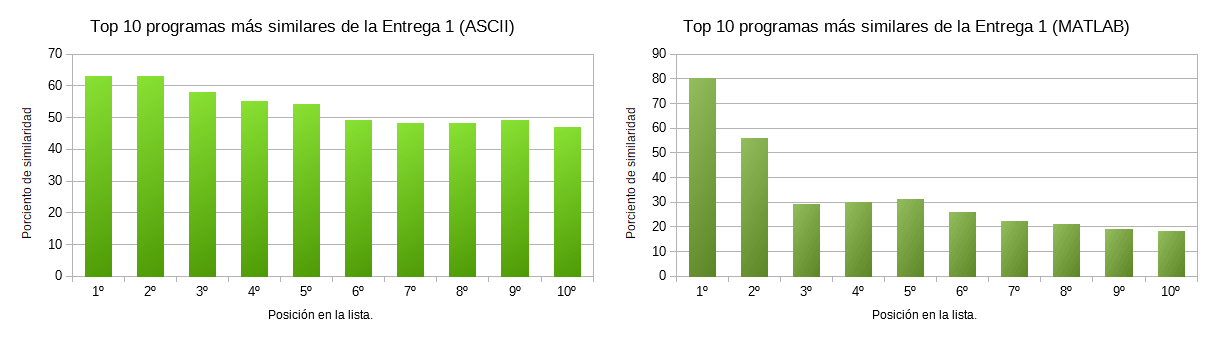
\includegraphics[width=14cm, height=6cm]{imagenes/TOP10_1.png}  %el parámetro scale permite agrandar o achicar la imagen. En el nombre de archivo puede especificar directorios
\caption{10 primeros pares de programas con mayor cantidad de código en común de la entrega 1} \label{fig:TOP10_1}
\end{figure}


Se puede apreciar que estos índices son más bajos que los obtenidos en JPLAG, esto en parte es debido a que MOSS ignora fragmentos de código que se repiten en al menos diez programas, lo que permite lidiar en cierta forma con los comentarios con el enunciado de los ejercicios (si es que al menos diez alumnos han decidido ponerlos).
\newline
Aun así, los resultados en modo texto plano (ASCII) sólo nos ayudan a encontrar programas con comentarios iguales o con código idéntico.
\newline
MOSS no encuentra tantas ocurrencias de plagio como nuestra versión de JPLAG, ya que se basa en un algoritmo que no tiene en cuenta los tokens si no un vector de características.
\newline
Lo que hace MOSS es tener en cuenta las palabras comunes del lenguaje elegido y en caso de aparecer no las considera plagio y no las tiene en cuenta en los índices de similaridad.
\newline
Los resultados obtenidos eligiendo como opción Matlab (ya que es el lenguaje mas parecido a R de los compatibles) son mejores que los de texto plano ya que nos han permitido encontrar algunas partes con sintaxis idéntica entre programas. De todas formas nuestro frontend de R ha encontrado estas mismas similaridades sintácticas además de una gran cantidad de plagio estructural y plagio en el que se cambia de orden el código o se añade código muerto, como en el caso de la Figura  \ref{fig:ENTREGA1_ESTRUCTURAL}, donde se ha encontrado un fragmento muy similar entre el código de los alumnos 1002 y 1036 que el resto de herramientas no ha detectado.

\bigskip
\begin{figure}[H] %con el [H] le obligamos a situar aquí la figura
\centering
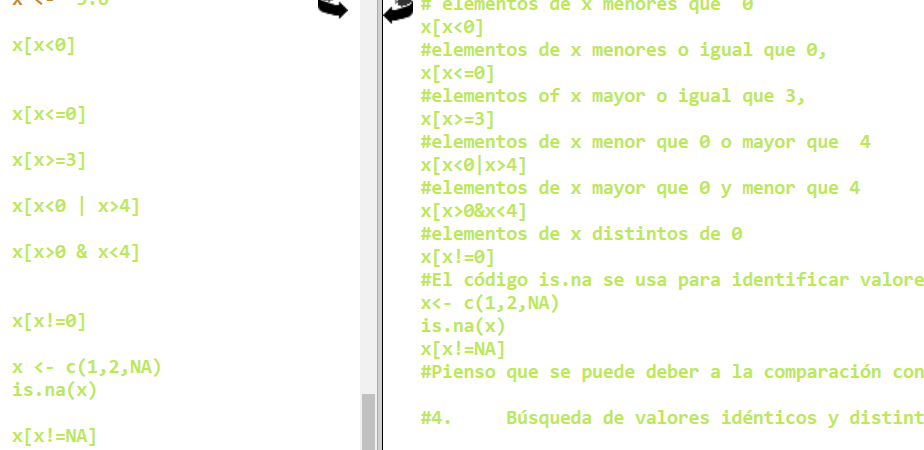
\includegraphics[width=8cm, height=5cm]{imagenes/ENTREGA1_ESTRUCTURAL.png}  %el parámetro scale permite agrandar o achicar la imagen. En el nombre de archivo puede especificar directorios
\caption{Ejemplo de plagio que sólo nuestro frontend ha encontrado en la primera entrega} \label{fig:ENTREGA1_ESTRUCTURAL}
\end{figure}

\bigskip
\bigskip


Las entregas 2 y 4 son muy similares ya que contienen ejercicios de uso de matrices, manipular y mostrar los datos que queramos de un dataset y manejo de factores(sólo en la 2), listas (sólo en la 4)y dataframes (sólo en la 4).
\newline
Ambas entregas son más del doble de largas que la primera entrega.
\newline

A continuación mostramos lás gráficas de los resultados para estas entregas (Figuras \ref{fig:histograma2}, \ref{fig:TOP10_2},\ref{fig:histograma4}, \ref{fig:TOP10_4}):

\begin{figure}[H] %con el [H] le obligamos a situar aquí la figura
\centering
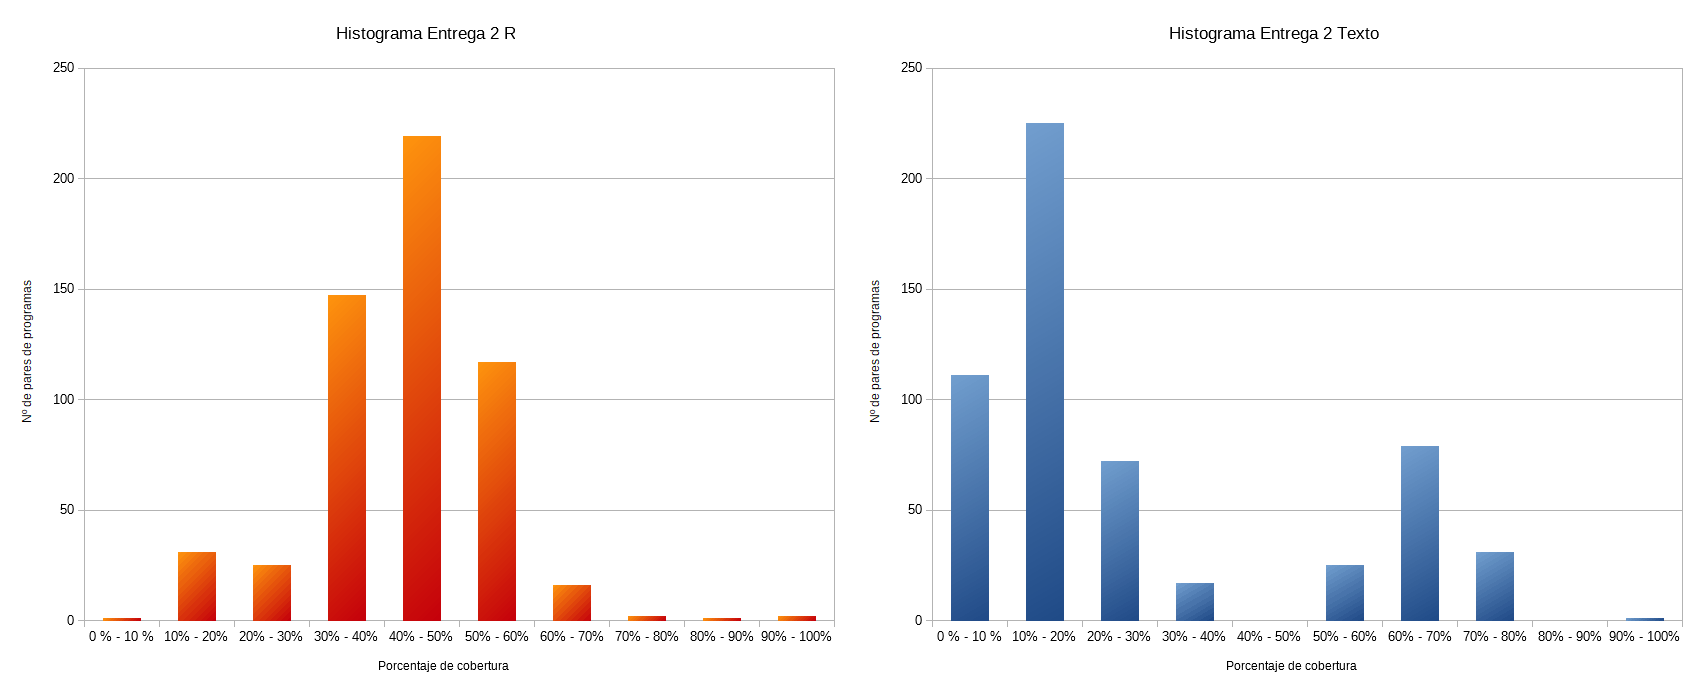
\includegraphics[width=15cm, height=7cm]{imagenes/histograma2.png}  %el parámetro scale permite agrandar o achicar la imagen. En el nombre de archivo puede especificar directorios
\caption{Histogramas de valores de similaridad entre todos los pares de programas de la segunda entrega.} \label{fig:histograma2}
\end{figure}


\begin{figure}[H] %con el [H] le obligamos a situar aquí la figura
\centering
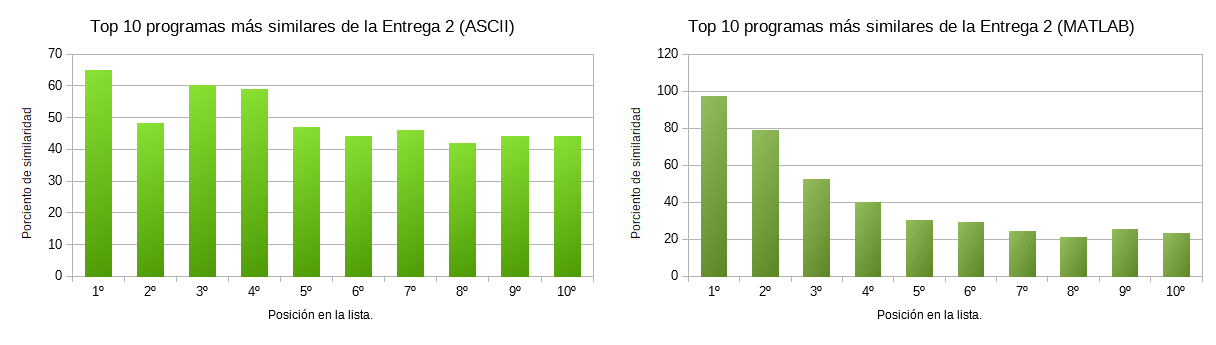
\includegraphics[width=14cm, height=6cm]{imagenes/TOP10_2.png}  %el parámetro scale permite agrandar o achicar la imagen. En el nombre de archivo puede especificar directorios
\caption{10 primeros pares de programas con mayor cantidad de código en común de la entrega 2} \label{fig:TOP10_2}
\end{figure}



\begin{figure}[H] %con el [H] le obligamos a situar aquí la figura
\centering
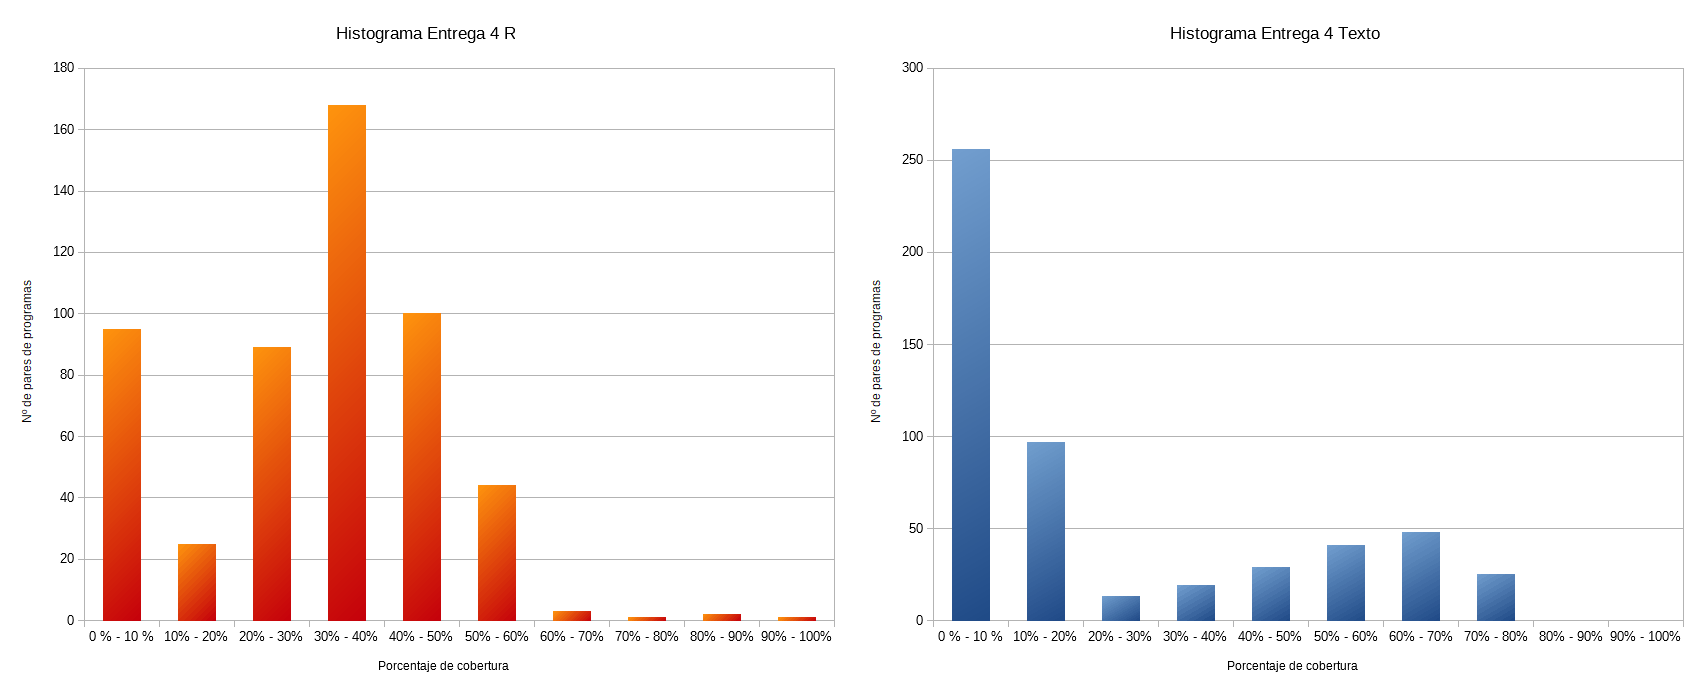
\includegraphics[width=15cm, height=7cm]{imagenes/histograma4.png}  %el parámetro scale permite agrandar o achicar la imagen. En el nombre de archivo puede especificar directorios
\caption{Histogramas de valores de similaridad entre todos los pares de programas de la cuarta entrega.} \label{fig:histograma4}
\end{figure}



\begin{figure}[H] %con el [H] le obligamos a situar aquí la figura
\centering
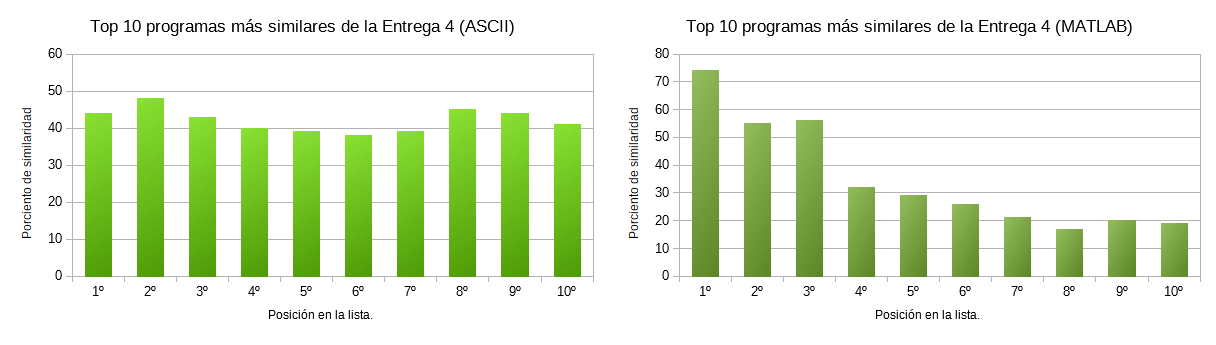
\includegraphics[width=14cm, height=6cm]{imagenes/TOP10_4.png}  %el parámetro scale permite agrandar o achicar la imagen. En el nombre de archivo puede especificar directorios
\caption{10 primeros pares de programas con mayor cantidad de código en común de la entrega 4} \label{fig:TOP10_4}
\end{figure}



Al consistir estas en programas más largos es más complicado que tengan una gran cantidad de código en común, es por esto que los histogramas de JPLAG y las gráficas de MOSS de estas entregas tienen índices de similaridad menores que los de la entrega 1.
\newline
Aún así JPLAG con nuestro frontend sigue encontrando bastantes pares con similaridad superior al 30\%. 

\bigskip
El resto de entregas son cortas pero obtenemos gráficas distintas debido a los ejercicios de cada una de estas:
\newline
La tercera y quinta entregas son algo distintas de lo visto hasta el momento, son entregas muy cortas con ejercicios similares; con 5 ejercicios de manipulación de strings en la tercera entrega y 5 ejercicios de E/S en la quinta.
\newline
Las gráficas de estas entregas se muestran a continuación(Figuras \ref{fig:histograma3}, \ref{fig:TOP10_3}, \ref{fig:histograma5}, \ref{fig:TOP10_5}):



\begin{figure}[H] %con el [H] le obligamos a situar aquí la figura
\centering
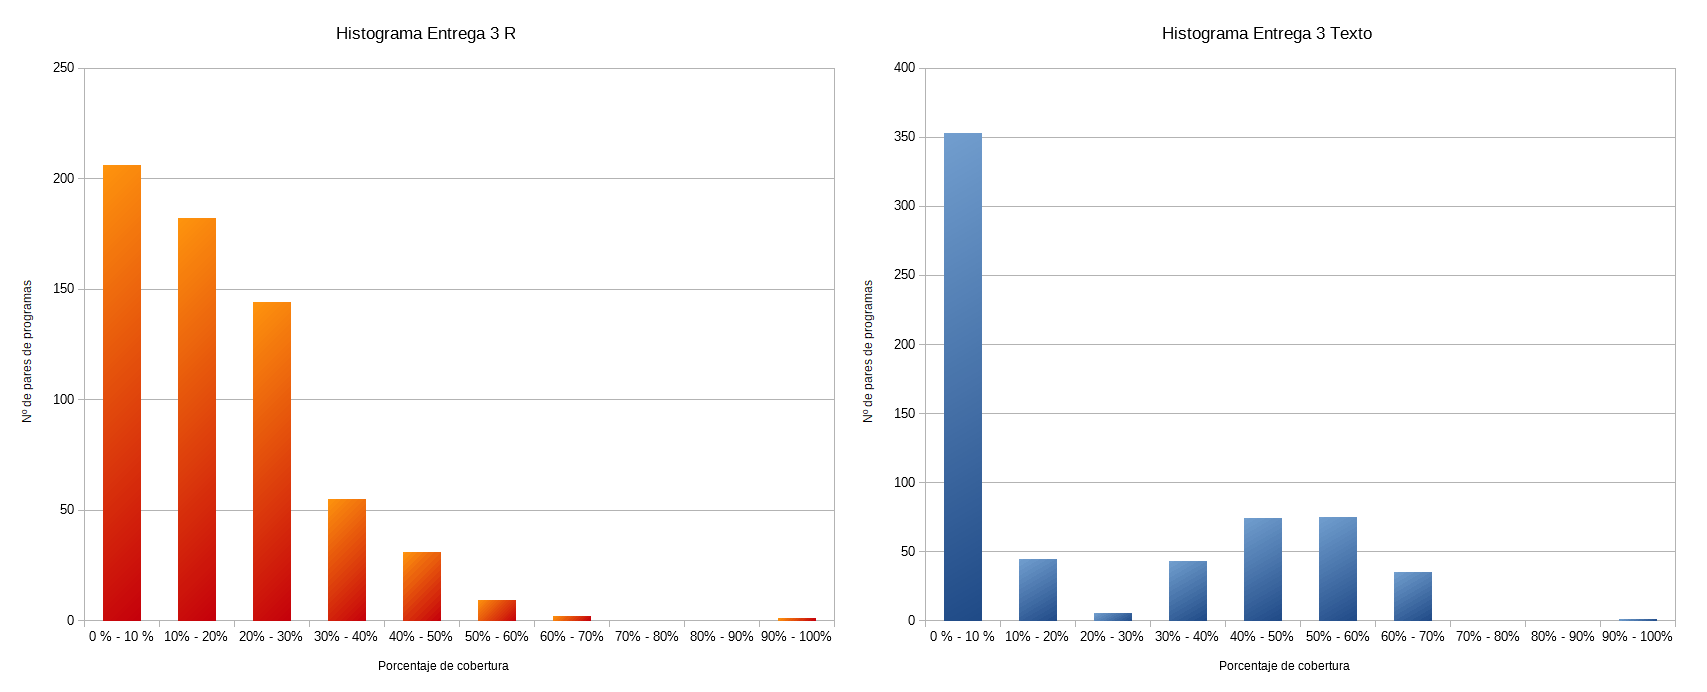
\includegraphics[width=15cm, height=7cm]{imagenes/histograma3.png}  %el parámetro scale permite agrandar o achicar la imagen. En el nombre de archivo puede especificar directorios
\caption{Histogramas de valores de similaridad entre todos los pares de programas de la tercera entrega.} \label{fig:histograma3}
\end{figure}


\begin{figure}[H] %con el [H] le obligamos a situar aquí la figura
\centering
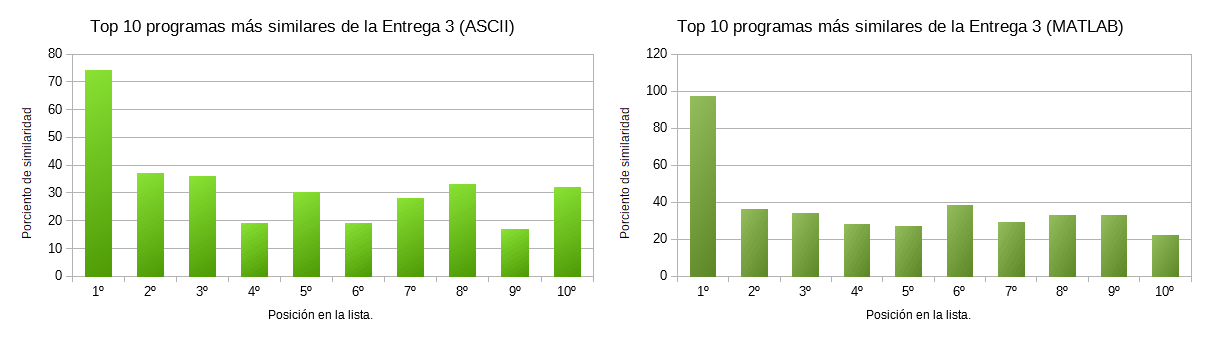
\includegraphics[width=14cm, height=6cm]{imagenes/TOP10_3.png}  %el parámetro scale permite agrandar o achicar la imagen. En el nombre de archivo puede especificar directorios
\caption{10 primeros pares de programas con mayor cantidad de código en común de la entrega 3} \label{fig:TOP10_3}
\end{figure}


\begin{figure}[H] %con el [H] le obligamos a situar aquí la figura
\centering
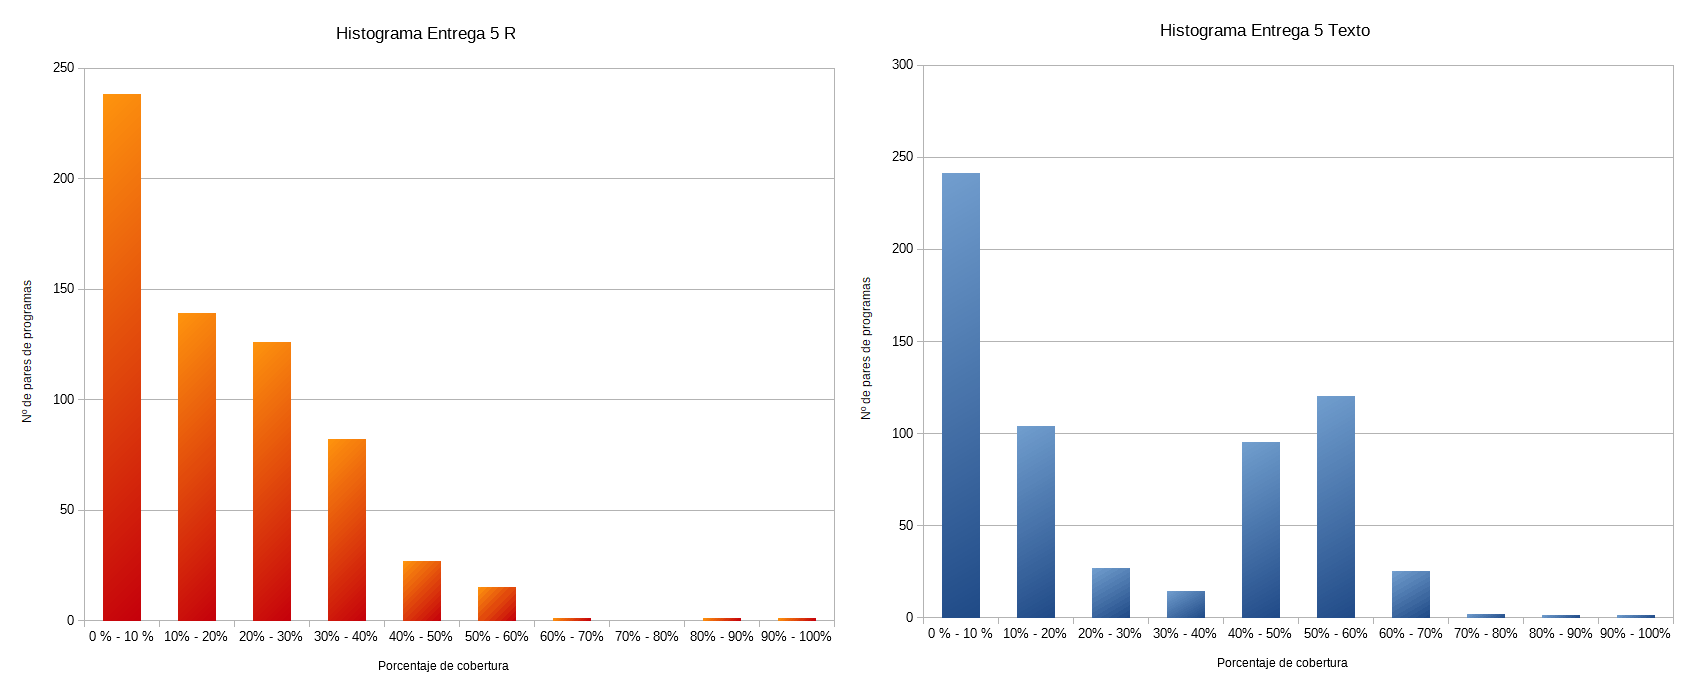
\includegraphics[width=15cm, height=7cm]{imagenes/histograma5.png}  %el parámetro scale permite agrandar o achicar la imagen. En el nombre de archivo puede especificar directorios
\caption{Histogramas de valores de similaridad entre todos los pares de programas de la quinta entrega.} \label{fig:histograma5}
\end{figure}





\begin{figure}[H] %con el [H] le obligamos a situar aquí la figura
\centering
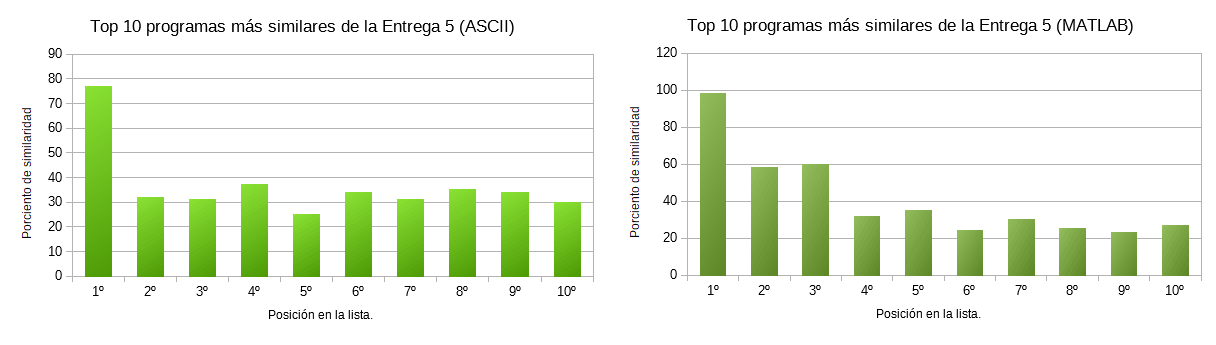
\includegraphics[width=14cm, height=6cm]{imagenes/TOP10_5.png}  %el parámetro scale permite agrandar o achicar la imagen. En el nombre de archivo puede especificar directorios
\caption{10 primeros pares de programas con mayor cantidad de código en común de la entrega 5} \label{fig:TOP10_5}
\end{figure}



Aún siendo ejercicios muy cortos los que se piden en estas entregas, estos se pueden abordar de numerosas formas, es por esto que los índices de similaridad detectados con JPLAG y MOSS entre estos pares de archivos son los más bajos hasta el momento.
\newline
Los pares detectados en MOSS y en JPLAG con texto con un índice superior al 40\% se deben a programas de alumnos que han escrito el enunciado de los ejercicios en su código, y al ser tan pocas las líneas de código que se requieren para hacerlo, los comentarios suponen más de un 50\% del documento en la mayoría de los casos.
\newline
Por otra parte, los contados casos en los que nuestro frontend ha detectado un alto porcentaje de cobertura entre emparejamientos se deben en su mayoría a alumnos que se han copiado pero han intentado ocultarlo cambiando el nombre de la variables, el de las cadenas de strings usadas y el de los documentos usados en los ejercicios de E/S.
Podemos ver un ejemplo de estos en Figura \ref{fig:ENTREGA5_variable}:


\begin{figure}[H] %con el [H] le obligamos a situar aquí la figura
\centering
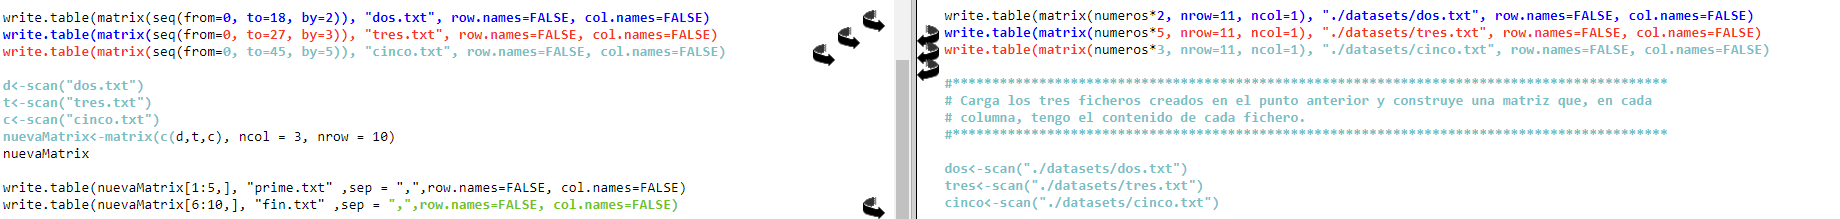
\includegraphics[width=15cm, height=5cm]{imagenes/ENTREGA5_variable.png}  %el parámetro scale permite agrandar o achicar la imagen. En el nombre de archivo puede especificar directorios
\caption{Ejemplo de plagio entre alumnos en el que se ha cambiado el nombre de variables y archivos(Entrega 5)} \label{fig:ENTREGA5_variable}
\end{figure}

\bigskip
Por último, en las entregas 6 y 7 se obtienen resultados similares a las entregas 3 y 5, ya que son igual de cortas, pero a diferencia de estas, tratan sobre ejercicios que requieren la definición de funciones. 
\newline
Para declarar una función como las que se piden en los ejercicios de estas entregas el alumno usará sus propias estructuras de control, variables y cálculos matemáticos.
\newline
Debido a esto se obtienen las siguientes gráficas de resultados (Figuras \ref{fig:histograma6}, \ref{fig:TOP10_6}, \ref{fig:histograma7}, \ref{fig:TOP10_7}):



\begin{figure}[H] %con el [H] le obligamos a situar aquí la figura
\centering
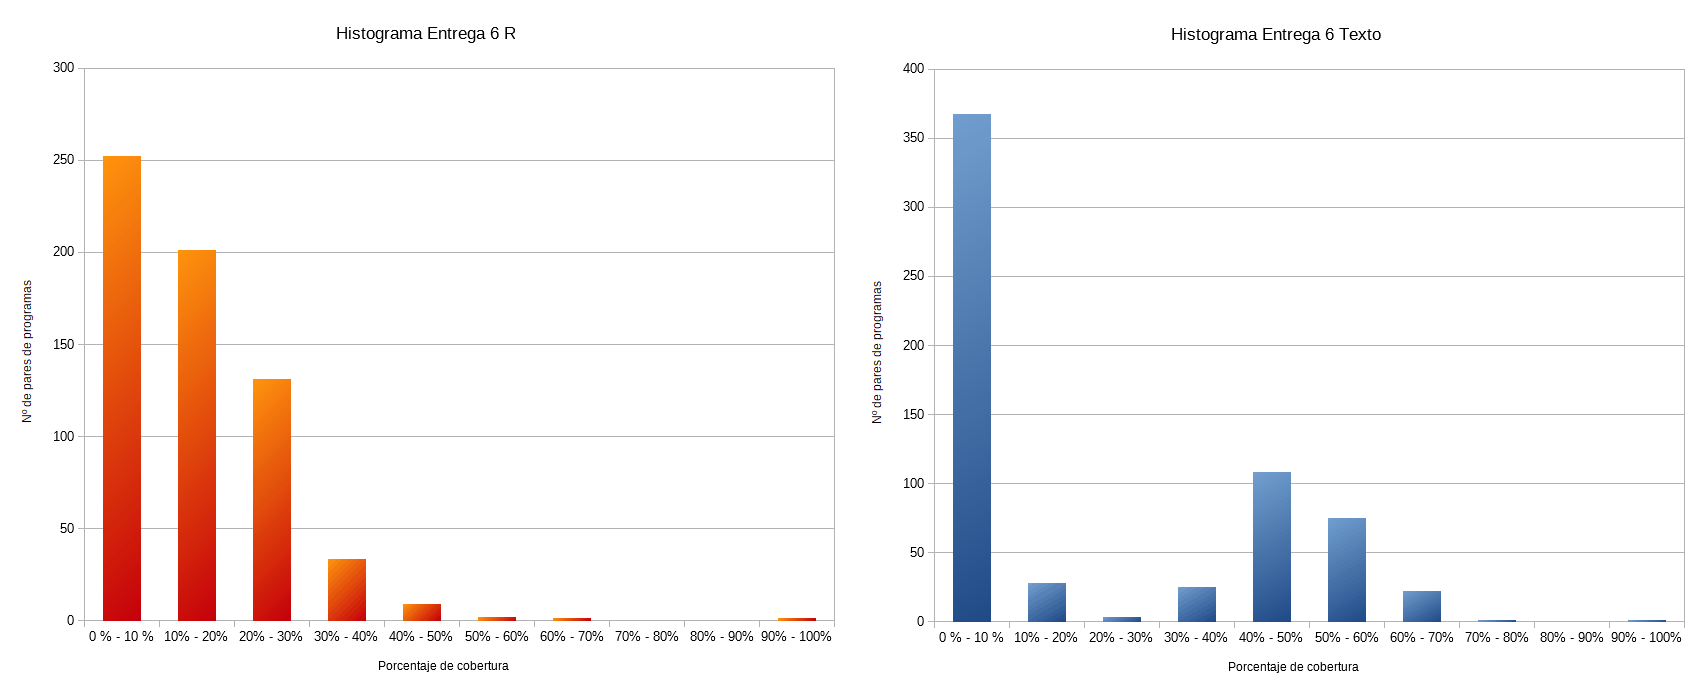
\includegraphics[width=15cm, height=7cm]{imagenes/histograma6.png}  %el parámetro scale permite agrandar o achicar la imagen. En el nombre de archivo puede especificar directorios
\caption{Histogramas de valores de similaridad entre todos los pares de programas de la sexta entrega.} \label{fig:histograma6}
\end{figure}



\begin{figure}[H] %con el [H] le obligamos a situar aquí la figura
\centering
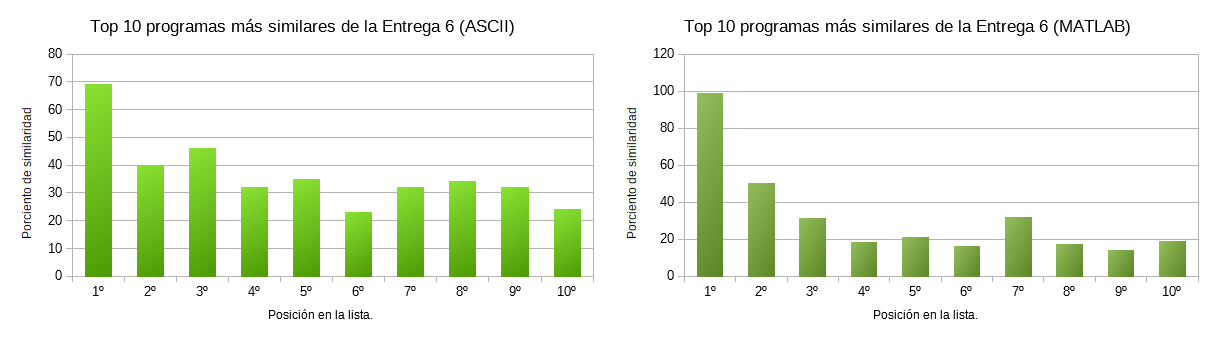
\includegraphics[width=14cm, height=6cm]{imagenes/TOP10_6.png}  %el parámetro scale permite agrandar o achicar la imagen. En el nombre de archivo puede especificar directorios
\caption{10 primeros pares de programas con mayor cantidad de código en común de la entrega 6} \label{fig:TOP10_6}
\end{figure}

\begin{figure}[H] %con el [H] le obligamos a situar aquí la figura
\centering
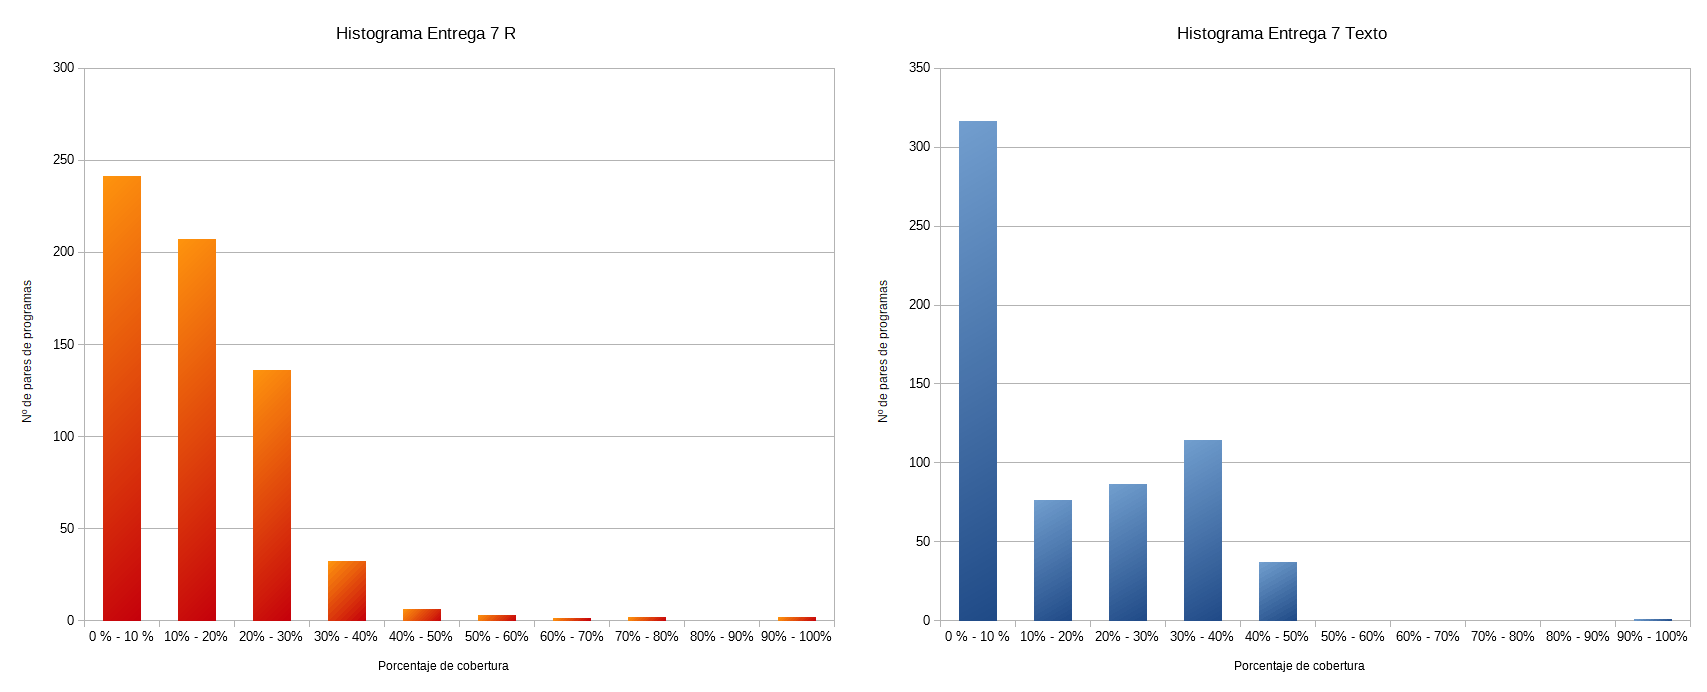
\includegraphics[width=15cm, height=7cm]{imagenes/histograma7.png}  %el parámetro scale permite agrandar o achicar la imagen. En el nombre de archivo puede especificar directorios
\caption{Histogramas de valores de similaridad entre todos los pares de programas de la séptima entrega.} \label{fig:histograma7}
\end{figure}




\begin{figure}[H] %con el [H] le obligamos a situar aquí la figura
\centering
\includegraphics[width=14cm, height=6cm]{imagenes/TOP10_7.png}  %el parámetro scale permite agrandar o achicar la imagen. En el nombre de archivo puede especificar directorios
\caption{10 primeros pares de programas con mayor cantidad de código en común de la entrega 7} \label{fig:TOP10_7}
\end{figure}


Los índices de similaridad son aún más bajos, los altos se deben a comentarios iguales como en los casos anteriores y nuestro frontend sigue detectando los contados plagios debidos a estructuras de control casí iguales.
\newline
\bigskip

Hemos podido comprobar en los resultados obtenidos en las siete entregas que el frontend que hemos creado para JPLAG permite detectar:
\begin{enumerate}
\item Plagios en los que el código se ha copiado entero.
\item Plagios en los que sólo se ha cogido parte del código.
\item Plagios en los que se ha modificado parcialmente el código para ocultar la copia, ya sea cambiando el nombre de variables o usando estructuras de control equivalentes.
\end{enumerate}
Pueden ocurrir falsos positivos con índice de similaridad alto, es por esto que los casos intermedios (entre 30\% y 60\% de similaridad) deben investigarse en mayor profundidad para comprobar si verdaderamente hay ocurrido plagio.
\newline
Para ello tan sólo tendremos que ir a las páginas de comparación de código donde se muestran los fragmentos donde se han detectado estructuras similares o iguales.
\newline
Los casos en los que ha ocurrido plagio y JPLAG con nuestro frontend no lo detecta requieren que el alumno haya modificado hasta tal punto la estructura del archivo que ya no se consideraría plagio, ya que esto significaría que el alumno entiende como funciona perfectamente el código que esta plagiando y sabe por tanto resolver el ejercicio.
















%
\chapter{Conclusiones y trabajo futuro}

\section{Conclusión}
En este trabajo hemos buscado y estudiado los orígenes del plagio y los recursos disponibles para su detección motivados por resolver el problema de la copia entre documentos en R.
\newline
Dado que en nuestra búsqueda no encontramos ninguna forma verdaderamente efectiva de detectar el plagio en este lenguaje, nos decidimos a resolver el problema modificando una de las mejores herramientas de detección de plagio llamada JPLAG.
\newline
Para ello, como ya explicamos en los capítulos de Elección de Herramientas e Implementación, ha sido necesario crear un frontend, adaptar un analizador sintáctico, elegir los tokens más importantes de R y comunicar todo con el programa principal.
\newline
Hemos comparado entonces la nueva herramienta creada con las mejores opciones existentes para detectar la copia entre alumnos.
\newline
Los resultados obtenidos de esta comparación han sido satisfactorios ya que nuestra herramienta, al contrario que el resto, consigue identificar prácticamente todos los casos de plagio entre alumnos, cosa imposible hasta el momento a menos que el profesor o evaluador hiciese todas las comparaciones manualmente.
\newline
\newline
Se han cumplido por tanto todos los objetivos que especificamos en un principio en el capítulo de introducción (Sección 1.3).


\section{Trabajo Futuro}

Aunque el trabajo hecho permite que sea posible detectar la mayor parte de los plagios en R entre tareas de alumnos, hay diversos añadidos que se pueden hacer para mejorar la herramienta:

\begin{itemize}
\item Basándonos en los detectores de plagio en documentos de texto como Turnitin y Viper, se podría añadir una base de datos de documentos para poder comparar los archivos enviados con archivos similares encontrados por internet o con las mismas entregas de alumnos de años anteriores. Para hacer esto se tendría que lidiar con la inmensa carga extra de trabajo que le supondría al algoritmo de comparación. En caso de poder solucionar ese problema, esto sería una gran mejora ya que permitiría saber si el alumno se ha copiado de un documento externo diferente al del resto de sus compañeros.
\item Aunque JPLAG ya tenga soporte para los lenguajes más usados, estaría bien añadir soporte para más lenguajes.
\item Entrenar una red neuronal con casos que son y no son plagio para que JPLAG pueda decir con un alto porcentaje de certeza si los casos que hasta el momento teníamos que inspeccionar con mayor profundidad(las casos intermedios) son plagio o no. Esto ahorraría un gran volumen de trabajo al evaluador.
\end{itemize}














%

%
%%\chapter{Conclusiones y Trabajos Futuros}
%
%
%%\nocite{*}
%\bibliography{bibliografia/bibliografia}\addcontentsline{toc}{chapter}{Bibliografía}
%\bibliographystyle{miunsrturl}
%

%\input{apendices/manual_usuario/manual_usuario}
%%\input{apendices/paper/paper}
%\input{glosario/entradas_glosario}
% \addcontentsline{toc}{chapter}{Glosario}
% \printglossary


%\thispagestyle{empty}

\bibliography{referencias} %archivo citas.bib que contiene las entradas 
\bibliographystyle{unsrt} % hay varias formas de citar

\appendix
\chapter{Código}

\section{RTokenConstants.java}
\lstinputlisting[inputencoding=latin1]{codigo/RTokenConstants.java}

\section{RToken.java}
\lstinputlisting[inputencoding=latin1]{codigo/RToken.java}


\section{Language.java}
\lstinputlisting[inputencoding=latin1]{codigo/Language.java}

\section{JplagRListener.java}
\lstinputlisting[inputencoding=latin1]{codigo/JplagRListener.java}

\section{Parser.java}
\lstinputlisting[inputencoding=latin1]{codigo/Parser.java}















\end{document}
